\documentclass[10pt,twocolumn,letterpaper]{article}

\usepackage{iccv}
\makeatletter
\@namedef{ver@everyshi.sty}{}
\makeatother
\usepackage{tikz}

\usepackage{times}
\usepackage{epsfig}
\usepackage{graphicx}
\usepackage{amsmath}
\usepackage{amssymb}
% \usepackage[usenames,dvipsnames]{xcolor}
\PassOptionsToPackage{usenames,dvipsnames}{xcolor}


\usepackage{booktabs}

\usepackage{soul}
\usepackage{enumitem}

\usepackage[pagebackref=true,breaklinks=true,letterpaper=true,colorlinks,bookmarks=false]{hyperref}

\iccvfinalcopy % *** Uncomment this line for the final submission

\def\httilde{\mbox{\tt\raisebox{-.5ex}{\symbol{126}}}}

\ificcvfinal\pagestyle{empty}\fi

\newcommand*{\ray}[1]{\textcolor{NavyBlue}{#1}}
\newcommand*{\bv}[1]{\textcolor{blue}{#1}}

\usepackage{tikz}
\usepackage{pgfplots}
\usepackage{ifthen}
\usetikzlibrary{
    fit,
    math,
    calc,
    arrows,
    shapes,
    shadows,
    fadings,
    external,
    plotmarks,
    arrows.meta,
    backgrounds,
    positioning,
    shadows.blur,
    intersections,
    pgfplots.groupplots,
    pgfplots.statistics,
    pgfplots.fillbetween,
}

\definecolor{b1}{HTML}{099CF0}
\definecolor{b2}{HTML}{0FA5C7}
\definecolor{yg}{HTML}{A1CB2E}
\definecolor{pg}{HTML}{5AAA4F}
\definecolor{or}{HTML}{F8A300}
\definecolor{pr}{HTML}{7000AD}
\definecolor{gr}{HTML}{EAEAF2}

\pgfdeclarelayer{back}
\pgfsetlayers{back,main}

\makeatletter
\pgfkeys{%
  /tikz/on layer/.code={
    \def\tikz@path@do@at@end{\endpgfonlayer\endgroup\tikz@path@do@at@end}%
    \pgfonlayer{#1}\begingroup%
  }%
}
\makeatother

\newcommand{\round}[2][2]{
    \pgfmathparse{#2}
    \pgfmathprintnumber[precision=#1, zerofill]{\pgfmathresult}
}

\makeatletter
\pgfplotsset{
    boxplot/hide outliers/.code={
        \def\pgfplotsplothandlerboxplot@outlier{}%
    }
}
\makeatother
\tikzexternalize[prefix=fig/external/]

\begin{document}

\renewcommand{\nu}{\ensuremath{\mathbf{n}(\mathbf{u})}\xspace}  % the normal vector at pixel location \V{u}
\newcommand{\pu}{\ensuremath{\mathbf{p}(\mathbf{u})}\xspace}   % the 3d point correspoinding the pixel \V{u}
\newcommand{\du}{\ensuremath{d(\mathbf{u})}\xspace}  
\newcommand{\zu}{\ensuremath{z(\mathbf{u})}\xspace}
\newcommand{\eu}{\ensuremath{\mathbf{e}(\mathbf{u})}\xspace}
\newcommand{\up}{\ensuremath{\V{u}_{\V{p}}}\xspace}
\newcommand{\tup}{\ensuremath{\tilde{\V{u}}_{\V{p}}}\xspace}

\newcommand{\oz}{\ensuremath{\Omega_z}\xspace}  
\newcommand{\on}{\ensuremath{\Omega_n}\xspace}
\newcommand{\Nu}{\ensuremath{\mathcal{N}(\V{u})}\xspace}

\renewcommand{\ni}{normal integration\xspace}
\newcommand{\NI}{Normal Integration\xspace}
\newcommand{\dpe}{discrete Poisson's equation\xspace}
\newcommand{\Dpe}{Discrete Poisson's equation\xspace}


\newcommand{\z}{\ensuremath{\V{z}}\xspace}
\newcommand{\zs}{\ensuremath{\V{z}^*}\xspace}
\newcommand{\rz}{\ensuremath{\red{\V{z}}}\xspace}
\newcommand{\zt}{\ensuremath{\V{z}_{t}}\xspace}
\newcommand{\zto}{\ensuremath{\V{z}_{t+1}}\xspace}
\newcommand{\R}{\ensuremath{\mathbb{R}}\xspace}
\newcommand{\fz}{\ensuremath{f(\V{z})}\xspace}

\newcommand{\rt}{\ensuremath{\V{r}_{t}}\xspace}
\newcommand{\rto}{\ensuremath{\V{r}_{t+1}}\xspace}


\newcommand{\dup}{\ensuremath{\V{D}_u^{+}}\xspace}
\newcommand{\dun}{\ensuremath{\V{D}_u^{-}}\xspace}
\newcommand{\dvp}{\ensuremath{\V{D}_v^{+}}\xspace}
\newcommand{\dvn}{\ensuremath{\V{D}_v^{-}}\xspace}
\newcommand{\nx}{\ensuremath{\V{n}_x}\xspace}
\newcommand{\ny}{\ensuremath{\V{n}_y}\xspace}
\newcommand{\nz}{\ensuremath{\V{n}_z}\xspace}
\newcommand{\Nz}{\ensuremath{\V{N}_z}\xspace}

\newcommand{\ft}{\ensuremath{F(\red{\V{z}};\V{z}_t)}\xspace}
\newcommand{\ftt}{\ensuremath{F(\V{z}_t;\V{z}_t)}\xspace}
\newcommand{\fto}{\ensuremath{F(\V{z}_{t+1};\V{z}_t)}\xspace}

\newcommand{\dpu}{\ensuremath{\partial_u \V{p}}\xspace}
\newcommand{\dpv}{\ensuremath{\partial_v \V{p}}\xspace}

\renewcommand{\u}{\ensuremath{\V{u}}\xspace}
\newcommand{\dzdu}{\ensuremath{\partial_u z}\xspace}
\newcommand{\dzdv}{\ensuremath{\partial_v z}\xspace}
\newcommand{\dztdu}{\ensuremath{\partial_u \tilde{z}}\xspace}
\newcommand{\dztdv}{\ensuremath{\partial_v \tilde{z}}\xspace}
\newcommand{\dzpdu}{\ensuremath{\partial_{u}^{+} z}\xspace}
\newcommand{\dzpdv}{\ensuremath{\partial_{v}^{+} z}\xspace}
\newcommand{\dzndu}{\ensuremath{\partial_{u}^{-} z}\xspace}
\newcommand{\dzndv}{\ensuremath{\partial_{v}^{-} z}\xspace}

\newcommand{\dzpduv}{\ensuremath{\partial_{\{u,v\}}^{+} z}\xspace}
\newcommand{\dznduv}{\ensuremath{\partial_{\{u,v\}}^{-} z}\xspace}
\newcommand{\dzduv}{\ensuremath{\partial_{\{u,v\}} z}\xspace}

\newcommand{\dupz}{\ensuremath{\Delta_{u}^{+} z}\xspace}
\newcommand{\dunz}{\ensuremath{\Delta_{u}^{-} z}\xspace}
\newcommand{\dvpz}{\ensuremath{\Delta_{v}^{+} z}\xspace}
\newcommand{\dvnz}{\ensuremath{\Delta_{v}^{-} z}\xspace}

\newcommand{\nuv}{\ensuremath{\V{n}(u,v)}\xspace}
\newcommand{\zuv}{\ensuremath{z(u,v)}\xspace}
\newcommand{\puv}{\ensuremath{\V{p}(u,v)}\xspace}

\newcommand{\halfpi}{\ensuremath{\pm {\pi \over 2}}\xspace}


\newcommand{\curve}{\ensuremath{\mathbb{S}}\xspace}
\newcommand{\zenith}{zenith\xspace}
\newcommand{\surface}{\ensuremath{\mathcal{M}}\xspace}
\newcommand{\visibility}{\ensuremath{\Phi_{i}}\xspace}
\newcommand{\point}{\ensuremath{\V{x}}\xspace}
\newcommand{\normal}{\ensuremath{\V{n}}\xspace}
\newcommand{\tangent}{\ensuremath{\V{t}}\xspace}
\newcommand{\cameraNum}{\ensuremath{C}\xspace}
\newcommand{\cameraCenter}{\ensuremath{\V{o}_{i}}\xspace}
\newcommand{\viewDirection}{\ensuremath{\V{v}}\xspace}
\newcommand{\batchsize}{\ensuremath{P}\xspace}
\newcommand{\mask}{\ensuremath{O}\xspace}
\newcommand{\projectedTangentVector}{projected tangent vector\xspace}
\newcommand{\projectedTangentVectors}{projected tangent vectors\xspace}
\newcommand{\stackedTangentVectors}{\ensuremath{\V{T}(\point)}\xspace}
\newcommand{\diligentmv}{\mbox{DiLiGenT-MV}\xspace}
\newcommand{\diligent}{DiLiGenT}
\newcommand{\loss}{\mathcal{L}\xspace}
\newcommand{\opticalAxis}{\ensuremath{\V{e}_{z}\xspace}}
\newcommand{\opticalAxisViewI}{\ensuremath{\V{e}_{z_{i}}}\xspace}
\newcommand{\opticalAxisMatrix}{\ensuremath{\V{C}}\xspace}
\newcommand{\ms}{Mumford-Shah integrator\xspace}
\newcommand{\made}{MADE\xspace}

\newcommand{\pandora}{\mbox{PANDORA}\xspace}
\newcommand{\psnerf}{\mbox{PS-NeRF}\xspace}
\newcommand{\sdps}{\mbox{SDPS}\xspace}
\newcommand{\uanet}{\mbox{UA-MVPS}\xspace}
\newcommand{\rmvps}{\mbox{R-MVPS}\xspace}
\newcommand{\bmvps}{\mbox{B-MVPS}\xspace}
\newcommand{\volsdf}{\mbox{VolSDF}\xspace}
\newcommand{\unisurf}{\mbox{UNISURF}\xspace}


\newcommand{\mvas}{MVAS\xspace}

\newcommand{\tsc}{\mbox{TSC}\xspace}

\newcommand{\pointOne}{\ensuremath{\point_1}\xspace}
\newcommand{\pointTwo}{\ensuremath{\point_2}\xspace}
\newcommand{\pointsetOne}{\ensuremath{\chi_{1}}\xspace}
\newcommand{\pointsetTwo}{\ensuremath{\chi_{2}}\xspace}
\newcommand{\fscoreThreshold}{\ensuremath{\tau}\xspace}
\newcommand{\chamferDist}{\ensuremath{d(\pointsetOne, \pointsetTwo)}\xspace}
\newcommand{\precision}{\ensuremath{\mathcal{P}}\xspace}
\newcommand{\recall}{\ensuremath{\mathcal{R}}\xspace}
\newcommand{\fscore}{\ensuremath{\mathcal{F}}\xspace}

\newcommand{\phaseangle}{\ensuremath{\hat{\phi}}\xspace}
\newcommand{\azimuthangle}{\ensuremath{\phi}\xspace}

\newcommand{\colorbar}[3]{
\begin{tabular}[t]{@{}l@{}l@{}}
	\includegraphics[height=#1\linewidth,width=0.5em]{colorbar.pdf} & 
	\begin{tabular}[b]{@{}l}
		#2 \\ [#3pt]
		$0$
	\end{tabular}
\end{tabular}
}



\setcounter{page}{1}
\title{Rethinking CycleGAN: Improving Quality of GANs for Unpaired Image-to-Image Translation}



\author{
    Dmitrii Torbunov, Yi Huang, Huan-Hsin Tseng, Haiwang Yu, \\Jin Huang, Shinjae Yoo, Meifeng Lin, Brett Viren, Yihui Ren\\
    Brookhaven National Laboratory, Upton, NY, USA\\
    % Upton, NY, USA\\
    {\tt\small \{dtorbunov,yhuang2,htseng,hyu,jhuang,sjyoo,mlin,bviren,yren\}@bnl.gov}
}

\maketitle
\ificcvfinal\thispagestyle{empty}\fi

\setlength{\abovedisplayskip}{5pt}
\setlength{\belowdisplayskip}{5pt}



Over the past few years, there has been a significant amount of research focused on studying the ReLU activation function, with the aim of achieving neural network convergence through over-parametrization. However, recent developments in the field of Large Language Models (LLMs) have sparked interest in the use of exponential activation functions, specifically in the attention mechanism.

Mathematically, we define the neural function $F: \R^{d \times m} \times  \mathbb{R}^d \rightarrow \mathbb{R}$ using an exponential activation function. Given a set of data points with labels $\{(x_1, y_1), (x_2, y_2), \dots, (x_n, y_n)\} \subset \mathbb{R}^d \times \mathbb{R}$ where $n$ denotes the number of the data. Here $F(W(t),x)$ can be expressed as $F(W(t),x) := \sum_{r=1}^m a_r \exp(\langle w_r, x \rangle)$, where $m$ represents the number of neurons, and $w_r(t)$ are weights at time $t$. It's standard in literature that $a_r$ are the fixed weights and it's never changed during the training. We initialize the weights $W(0) \in \mathbb{R}^{d \times m}$ with random Gaussian distributions, such that $w_r(0) \sim \mathcal{N}(0, I_d)$ and initialize $a_r$ from random sign distribution for each $r \in [m]$.

Using the gradient descent algorithm, we can find a weight $W(T)$ such that $\| F(W(T), X) - y \|_2 \leq \epsilon$ holds with probability $1-\delta$, where $\epsilon \in (0,0.1)$ and $m = \Omega(n^{2+o(1)}\log(n/\delta))$. To optimize the over-parametrization bound $m$, we employ several tight analysis techniques from previous studies [Song and Yang arXiv 2019, Munteanu, Omlor, Song and Woodruff ICML 2022]. 

 

\section{Introduction}

The increasing complexity of source code poses a key challenge to the reliability of large-scale software systems. Software bugs in these systems can lead to safety issues~\cite{bug_safety} for users around the world as well as cause non-negligible financial losses~\cite{bug_loss}. As such, developers have to spend a large amount of time and effort on bug fixing. Consequently, \aprfull (\apr), designed to automatically generate patches to fix software bugs, has attracted wide attention from both academia and industry~\cite{long2016prophet, legoues2012genprog, long2015spr, lou2020can, tufano2018empstudy}. 


To achieve \apr, one popular approach is known as Generate-and-Validate (G\&V)~\cite{qi2015gv, ghanbari2019prapr, lou2020can, le2016hdrepair, legoues2012genprog, wen2018capgen, hua2018sketchfix, martinez2016astor, koyuncu2020fixminder, liu2019tbar, liu2019avatar}, which is typically based on the following pipeline: First, fault localization techniques~\cite{wong2016fl, abreu2007ochiai, zhang2013injecting, papadakis2015metallaxis, li2019deepfl, li2017transforming} are applied to determine the suspicious locations in programs where bugs are likely to exist. Then, the buggy locations are used by the \apr tools to generate a list of patches that replace buggy lines with correct lines. Afterward, each patch is validated against the original test suite to identify any \emph{plausible patches} (i.e., passing all tests in the test suite). Finally, to determine the \emph{correct patches}, developers examine the list of plausible patches to see if any of them can correctly fix the bug. 

Traditional \apr tools can mainly be categorized into heuristic-based~\cite{legoues2012genprog, le2016hdrepair, wen2018capgen}, constraint-based~\cite{mechtaev2016angelix, le2017s3, demacro2014nopol, long2015spr} and \template~\cite{ghanbari2019prapr, hua2018sketchfix, martinez2016astor, liu2019tbar, liu2019avatar}. Among these traditional tools, \template \apr tools~\cite{ghanbari2019prapr, liu2019tbar, benton2020effectiveness} have been able to achieve state-of-the-art results. \Template \apr tools typically leverage pre-defined templates (e.g., adding a nullness check) for bug fixing. However, since these fix templates are typically handcrafted, the number and types of bugs they are able to fix can be limited. 



To address the limitations of traditional \apr, researchers have proposed various \learning \apr tools~\cite{li2020dlfix, chen2018sequencer, jiang2021cure, lutellier2020coconut, zhu2021recoder, ye2022rewardrepair} based on the \nmtfull (\nmt) architecture~\cite{sutskever2014mt} where the input is the buggy code snippets and the goal is to translate the buggy code snippets into a fixed version. To accomplish this, \learning \apr tools require supervised training datasets with pairs of both buggy and fixed code snippets in order to learn how to perform this translation step. These training data are usually obtained by mining historical bug fixes using heuristics/keywords~\cite{dallmeier2007benchmark}, which can be imprecise for identifying bug-fixing commits; even the actual bug-fixing commits can include irrelevant code changes, leading to further pollution in the dataset~\cite{xia2022alpharepair}.
% 
Moreover, it can be hard for such \apr tools to generalize and fix bug types unseen during training. 



To better leverage recent advances in \plmfull{s} (\plm{s}), researchers~\cite{xia2022alpharepair, xia2023repairstudy, kolak2022patch, prenner2021codexws} have directly applied \plm{s} to generate patches without bug-fixing datasets. These \llm-based \apr tools work by either directly generating a complete code function~\cite{prenner2021codexws, xia2023repairstudy} or predict/infill the correct code snippet given its surrounding context~\cite{xia2022alpharepair, xia2023repairstudy}. By directly using \llm{s} that are pre-trained on billions of open-source code snippets, \llm-based \apr tools can achieve state-of-the-art performance on many repair datasets~\cite{xia2022alpharepair}. 


% 
%
%

Traditional \apr tools have long used the insight of the \emph{plastic surgery hypothesis}~\cite{barr2014plastic} where it states that the code ingredients to fix a bug already exist within the same project. Traditional \apr tools have manually designed pattern-~\cite{ghanbari2019prapr, saha2017elixir} or heuristic-based~\cite{jiang2018simfix, legoues2012genprog} approaches to finding and using such relevant code ingredients to generate fixes for bugs. However, the plastic surgery hypothesis has been largely ignored in \llm-based \apr. In fact, \llm provides a unique opportunity to fully automate the plastic surgery hypothesis idea via fine-tuning (learning project-specific information via model updates from the buggy project) and prompting (directly providing relevant code ingredients to the model), and make it directly applicable to different languages (since the \llm{s} are typically multi-lingual).%
Moreover, despite the intensive manual efforts involved, traditional \apr tools still cannot fully leverage project-specific information due to large search space for leveraging/composing existing code ingredients. In contrast, the project-specific information can effectively leveraged by \llm{s} due to their power in code understanding/vectorization, e.g., even partial/imprecise information may still guide \llm{s} in correct patch generation!
 To this end, we ask the question: \emph{How useful is the plastic surgery hypothesis in the era of \plm{s}}?








\mypara{Our Work.} To answer the question, we present \ourtech{\xspace} -- a \llm-based approach that automatically utilizes the plastic surgery hypothesis by systematically combining multiple fine-tuning and prompting strategies for \apr. \ourtech fine-tunes \plm{s} using two novel domain-specific training strategies: \textbf{\epfinetune} -- we fine-tune using the original buggy project by aggressively masking out a high percentage of tokens, which allows \plm to learn project-specific code tokens and programming styles; and \textbf{\rofinetune} -- which only masks out a single continuous code sequence per training sample, allowing the model to get used to the final \csapr task of predicting a single continuous code sequence. Furthermore, we directly leverage the ability for \plm{s} to understand natural language instructions and introduce a novel prompting strategy, \textbf{\idprompting}, which uses information retrieval and static analysis to obtain a list of relevant identifiers for the buggy lines. While such relevant identifiers are critical for fixing some difficult bugs, they may not be seen by the \llm during inference due to limited context window size. Through the use of prompting, we directly tell the model to use these extracted identifiers (relevant code ingredients) to generate the correct code. Finally, to perform repair, we combine all four model variants (including the base model, both fine-tuned models and the base model with prompting) for the final repair.





While our insight of leveraging the plastic surgery hypothesis for \llm-based \apr is generalizable across different types of \plm{s}, to implement \ourtech, we choose a recent \plm{\xspace}, \ctfive~\cite{wang2021codet5}, which is pre-trained on millions of open-source code snippets. \ctfive is an encoder-decoder model trained using \mspfull (\msp) objective where a percentage of tokens are masked out and each continuous masked token sequence is referred to as a masked span. Also, although we only extract relevant identifiers from the current buggy project (since this paper focuses on the plastic surgery hypothesis), our work can be easily extended to obtain other code information (such as relevant statements or functions) from other sources, such as  the massive pre-training corpora~\cite{husain2020codesearchnet} or historical bug-fixing datasets~\cite{jiang2019infer}, which can provide more coding knowledge for \llm{s}. Besides, although we mainly focus on using traditional string comparison algorithms for information retrieval in this paper, these techniques can be easily replaced by other frequency-based retrieval~\cite{robertson2009probabilistic} and neural search (or embedding-based search)~\cite{reimers2019sentence}.
  In summary, this paper makes the following contributions:


%


\begin{itemize}[noitemsep, leftmargin=*, topsep=0pt]
    \item \textbf{Dimension.} This paper is the first to revisit the important plastic surgery hypothesis in the era of \llm{s}. It opens up a new dimension for \llm-based \apr to incorporate previously neglected information from the buggy project itself to boost \apr performance. Furthermore, it demonstrates the promising future of retrieval-based prompting for modern \llm-based \apr.
    \item \textbf{Implementation.} We implement \ourtech based on the recent \ctfive model. We augment the model using two novel fine-tuning strategies: \epfinetune and \rofinetune, along with a novel prompting strategy based on information retrieval and static analysis: \idprompting. We combine the patches generated by all four models together and perform patch ranking to speed up \apr.% 
    \item \textbf{Evaluation Study.} We conduct an extensive evaluation against state-of-the-art \apr tools. On the widely studied \dfj 1.2 and 2.0 datasets~\cite{just2014dfj}, \ourtech is able to achieve the new state-of-the-art results of 89 and 44 correct bug fixes (15 and 8 more than best baseline) respectively.  Furthermore, we perform a broad ablation study to justify our design. \ourtech demonstrates for the first time that the plastic surgery hypothesis can substantially boost \llm-based \apr and advance state-of-the-art \apr, while being fully automated and general. Moreover, even partial/imprecise code ingredients may still effectively guide \llm{s} for \apr!
\end{itemize}


\section{Related work}
% There is extensive recent work on speeding up analytical queries due to the need for consistent execution times in the face of the explosive growth in the volume of available data.
% In this section, we divide existing work into two categories: maintaining data freshness in MVs (\Cref{sec:server_side}) and optimizations for minimizing ad-hoc query latency (\Cref{sec:client_side}).

% \subsection{Maintaining Data Freshness in MVs}
% \label{sec:server_side}
% There exists a variety of data warehousing applications aimed at supporting low-latency analytical queries on fresh data.
% In particular, these applications require efficiency in the propagation of newly ingested data into downstream MVs.
 
\mypara{Efficient MV Refresh}
Incremental view maintenance (IVM) aims to update MVs to reflect newly ingested data, taking advantage of already computed results to perform the update in a manner more efficient than computing from scratch (full refresh)
~\cite{ahmad2012dbtoaster,mcsherry2013differential,armbrust2013generalized,zeng2016iolap, palpanas2002incremental, griffin1995incremental, agiwal2021napa, braun2015analytics}. 
There is an abundance of work in IVM, including incremental updates on duplicate values~\cite{griffin1995incremental}, non-distributive aggregate functions~\cite{palpanas2002incremental}, higher-order views~\cite{ahmad2012dbtoaster}, and sliding windows~\cite{braun2015analytics}. 
More recent works also investigate the scalability aspect of IVM, proposing scale-independent updates~\cite{armbrust2013generalized} and sampled views~\cite{zeng2016iolap}. Since \system is applicable to arbitrary SQL statements, \system is orthogonal to and is fully compatible with existing IVM techniques.

\mypara{MV Refresh Scheduling}
There exist works on scheduling the refresh of a MV set focusing on resolving cyclic dependencies~\cite{folkert2005optimizing}, minimizing weighted average staleness~\cite{golab2009scheduling}, and prioritizing MVs with the highest speedups on predicted future queries~\cite{ahmed2020automated}.
\system's scheduling to speed up the end-to-end refresh of the MV set is not addressed in existing works.

\mypara{DAG Workflow Scheduling}
The execution of workloads consisting of individual jobs with acyclic dependencies is a well-studied topic~\cite{apacheoozie,sparkdag,marchal2018parallel,bathie2020revisiting,baruah2022ilp}; many of these techniques can be applied to MV refresh runs studied in this paper.
Existing workflow scheduling systems such as Apache Oozie~\cite{apacheoozie}, Apache Airflow~\cite{airflow}, and Spark DAG scheduler~\cite{sparkdag} automate the execution of user-defined workflows following a topological order.
There are recent works aimed at finding more optimal execution orders in terms of peak memory usage~\cite{marchal2018parallel, bathie2020revisiting} and execution time on parallel platforms~\cite{baruah2022ilp}.
While \system is designed for use with MV refresh runs/workloads, our technique on joint scheduling and optimization can be reasonably applied to general workloads as a possible future direction.

% \paragraph{Incremental MV indexing}
% Update-optimized indices such as the log-structured merge-trees (LSM)~\cite{o1996log} are used for indexing MVs due to frequent updates induced by data ingestion~\cite{gupta2016mesa,agiwal2021napa}.
% \system is orthogonal to indexing: \system is capable of efficiently performing MV refresh runs regardless of whether the individual MVs are indexed or not.

% \subsection{Ad-hoc Query Latency Reduction}
% \label{sec:client_side}

% The minimization of ad-hoc analytical query response times is a well-studied topic due to latency being negatively correlated with the productivity of a data analyst during a data analysis session~\cite{liu2014effects}.
% Sessions are commonly conducted within visualization systems that contain a variety of optimization techniques to ensure that query response times fall within a certain latency tolerance.

% \mypara{Data prefetching}
% Data is often loaded into memory on a by-need basis in visualization systems to minimize interference with user-issued query computations~\cite{mani2017effective,xin2021enhancing,galakatos2017revisiting, yan2020auto, battle2016dynamic, crotty2016case, jalaparti2018netco}. 
% Query-time data retrieval can be significantly expedited by anticipating the data usage of the user in future queries and pre-loading the data into memory during the downtime between user queries (`think time'). SMART~\cite{mani2017effective} prefetches data for modified versions of current user-issued queries with different filters and dimensions. A-WARE~\cite{crotty2016case} maintains a sample store constantly refined through ingesting data based on speculations of future plots.
% ForeCache~\cite{battle2016dynamic} uses an SVM to predict the user's current analysis phase and accordingly prefetches data tiles partitioned based on different numerical values. NetCo predicts future queries via log analysis, and solves an ILP formulation to prefetch data to maximize the number of SLO-meeting queries~\cite{jalaparti2018netco}.
% In the case of MV refresh workloads, `think time' is nonexistent as individual MVs are refreshed back-to-back, rendering data prefetching techniques non-applicable.

\mypara{Intermediate Data Caching}
Some existing data visualization systems cache user-defined variables to support the typical incremental construction of data visualizations~\cite{zgraggen2016progressive, eichmann2020idebench} during data analysis sessions~\cite{jupyter, rstudio, colab}. 
Recent work proposes a management scheme for these cached variables under a memory constraint that greedily keeps variables with the highest estimated time savings based on predicted future user behavior via neural networks~\cite{xin2021enhancing}.
While useful for data visualization, a greedy approach to memory management fails to achieve satisfactory results compared to \system.

\mypara{Intermediate Result Reuse}

There exist works on storing intermediate results from computations to speedup future computations~\cite{yang2018intermediate, dursun2017revisiting, nagel2013recycling, michiardi2019memory, galakatos2017revisiting}.
Studied topics include the identification of reuse opportunities by finding overlaps in computation graphs of successive jobs~\cite{yang2018intermediate, michiardi2019memory},
selective storage under a space constraint with heuristics such as reuse probability~\cite{dursun2017revisiting}, expected savings~\cite{yang2018intermediate}, and recompute-storage cost difference~\cite{nagel2013recycling},
and rewriting incoming jobs to take advantage of stored intermediates~\cite{galakatos2017revisiting}.
These works share similarity with \system in their selection of items to store under a memory constraint, however, \system's problem setting requires it to uniquely consider the joint (re)ordering of job executions along with the selection of items.

% work that considers both job execution (re)order as well as intermediate result caching with a bounded amount of memory. but notably lack the joint aspect of \system and cannot be used to achieve immediate speedup on an incoming MV refresh run if no intermediates are stored beforehand. 

\mypara{Incremental Query Processing} Incremental processing (IQP) is useful for cases where not all data required for a query is immediately available. Similar to online aggregation~\cite{hellerstein1997online}, initial results of a query are computed on a subset of required data and progressively refined as the rest of the required data arrives in a predictable pattern~\cite{tang2019intermittent,wangtempura}. Tang et al. propose a dynamic programming formulation to pick intermediate states to store in memory given a limited memory budget~\cite{tang2019intermittent}. Tempura rewrites the query plan for more efficient execution based on predicted data arrival patterns~\cite{wangtempura}. While similarities exist between the problem setting of IQP and \system, such as management of bounded memory, \system notably includes additional joint optimization for the order of MV updates.

% \paragraph{Sampling}
% Sampling has seen wide use in visualization systems for reducing the computation time of ad-hoc queries by computing an approximate result over a subset of data as exact results are not always required by the user~\cite{crotty2016case, mani2017effective, zgraggen2014panoramicdata, kraska2021northstar, galakatos2017revisiting, kandula2016quickr}. 
% Commonly studied topics in sampling for ad-hoc queries include complex query sampling~\cite{kandula2016quickr}, rare event aggregation~\cite{kraska2021northstar, galakatos2017revisiting}, and maintaining consistency between related sampled visualizations~\cite{zgraggen2014panoramicdata}.
% Sampling server-side at the MV level compromises the assumptions of downstream applications and is thus not considered in \system.

% \paragraph{Progressive visualization}
% The latency tolerance for time-consuming queries can be circumvented by presenting a partially-computed visualization to the user within the tolerance, which is then incrementally refined until it is fully accurate~\cite{rahman2017ve, zgraggen2016progressive, crotty2015vizdom, kraska2021northstar, kamat2017infiniviz}.
% Example plots which benefit from progressive visualization include bar charts~\cite{kamat2017infiniviz} and heatmaps~\cite{rahman2017ve}.
% Similar to sampling, study on this topic is orthogonal to \system as pushing out partially-updated MVs compromises downstream assumptions.
\section{Method}
\label{sec:method}

% \ml{``Inconsistent'' to ``large variation''}

% In this section, we propose our methods based on the observations in Section \ref{sec:motivation}.
In this section, we propose two techniques to further enhance the strong baseline to capture the variation of activation distributions better.
We first introduce spatial re-scaling to adapt the network to pixel-to-pixel variation.
We then propose channel-wise shifting and re-scaling to better capture the channel-to-channel variation.
Meanwhile, as both of the two methods are image-dependent, the image-to-image variation can be captured naturally.
By combining the two methods with our strong baseline, we build our enhanced BNN for SR, named EBSR.

% Because the activation distributions among pixels, channels and images have large variations \red{**are highly inconsistent} in SR networks, we introduce spatial re-scaling to adapt to pixel-wise variations and channel shift and re-scaling to adapt to channel-wise variations. And both of them are image-dependent to adapt to image-wise variations, which means during inference our network re-scales and shifts the distributions of activations flexibly for different input images. Based on these methods, we build an enhanced binary neural network for image super-resolution (EBSR).

% According to [3], the difference of activation magnitudes indicates different scaling factors are needed for each pixel.

\subsection{Spatial Re-scaling}
% It is better to use different scaling factors for different pixels to reduce the quantization error and retain more detailed information for image super-resolution. 

% \ml{In the main method, we do not need to introduce the previous works but can focus on introducing our own method. Channel rescaling in Real-to-binary Net is not relevant in this context.}

% Re-scaling the output of binary convolutions was proposed at the birth of BNN in XNOR-Net \cite{rastegari2016xnor} to reduce quantization error and improve accuracy for image classification tasks.
% It is computed as below:
% \begin{equation}
% \mathcal{A} * \mathcal{W} \approx(\operatorname{sign}(\mathcal{A}) \circledast \operatorname{sign}(\mathcal{W})) \odot \mathcal{K} \alpha
% \label{eq:xnor-net rescale}
% \end{equation}
% where $\circledast$ denotes the binary convolution and $\odot$ denotes the element-wise multiplication.
% $\mathcal{A}$, $\mathcal{W}$, $\alpha$, and $\mathcal{K}$ denote the activation, weight, weight scaling factor, and activation scaling factor, respectively.
%  Later in XNOR-Net++ \cite{bulat2019xnor}, Bulat et al. fuse the activation and weight scaling factors into a single one that is learned end-to-end based on gradients and this improves the classification accuracy on ImageNet dataset.

% % It is computed as Eq.~\ref{eq:xnor-net rescale}, where $\circledast$ denotes 
% %  the binary convolution and $\odot$ denotes the element-wise multiplication. The binary convolution of $\mathcal{A}$ and $\mathcal{W}$ is rescaled by the weight scaling factor $\alpha$ and the activation scaling factor $\mathcal{K}$, both of which are calculated analytically.


% \zc{Similarly, you should explain the meaning of A, W and the operators $\circledast$ in the formula}
% Then in Real-to-binary Net \cite{martinez2020training}, Martinez et al. used a data-driven channel re-scaling module that takes the pre-convolution activations as input to predict the activation scaling factor. Unlike that in XNOR-Net++ \cite{bulat2019xnor}, these scaling factors are not fixed during inference but rather inferred from data. By doing this, they further improved the classification accuracy on ImageNet over XNOR-Net++. 
As is shown in Figure \ref{fig:pixel}, activation distributions have large pixel-to-pixel variation in SR networks
and the difference of activation magnitudes indicates different scaling factors are preferred for different pixels.
Inspired by \cite{martinez2020training}, we propose spatial re-scaling to better adapt the network to the spatial variation
of activation distributions in SR networks.
% fit the various pixel-wise distributions in SR networks.
We take the real-valued activations $A$ before convolution as input and predict pixel-wise scaling factors $S(A)$, which re-scale the binary convolution output. Spatial re-scaling process can be formulated as follows:
\begin{equation}
A * W \approx(\operatorname{sign}(A) \circledast \operatorname{sign}(W)) \odot \alpha \odot S(A)
\label{eq:spatial rescale}
\end{equation}
where $\circledast$ denotes 
the binary convolution and $\odot$ denotes the element-wise multiplication. $A$, $W$, $\alpha$, and $S\left(A\right)$ denote real-valued activations, weights, the scaling factor of weights, and the spatial-wise scaling factor of activations respectively. $S\left(A\right) \in \mathbb{R}^{1\times H\times W}$ can be calculated with a convolution and a sigmoid function.
% as $\sigma\left( CONV\left(A\right)\right)$. 
As shown in Figure \ref{fig:method}(a), real-valued activations first go through a convolution layer,
which has an input channel of $C$ and an output channel of 1, 
and then pass through a sigmoid function to produce the scaling factors $S(A)$ along the spatial dimension.
During inference, the scaling factor will change dynamically according to different input feature maps.
By re-scaling binary convolution output using $S(A)$, we can reduce the quantization error and the original pixel-wise information in FP activation
will be preserved much better.
Spatial re-scaling leads to a large PSNR improvement of 0.24 dB (from 30.30 dB to 31.54 dB) on Set5 and 0.22 dB (from 25.09 dB to 25.31 dB)
on Urban100 compared with our strong baseline. 

\subsection{Channel-wise Shifting and Re-scaling}

\begin{table}[!tb]
\centering
\caption{Comparison between whether to fuse channel-wise shifting and re-scaling or not based on our baseline with spatial re-scaling. }
\label{tab:fusing}

\scalebox{0.65}{
\begin{tabular}{c|cc|cc|cc}
\hline
\multirow{2}{*}{Method}     & \multirow{2}{*}{OPs} & \multirow{2}{*}{Params} & \multicolumn{2}{c|}{Set5} & \multicolumn{2}{c}{Urban100} \\ \cline{4-7} 
                            &                      &                         & PSNR        & SSIM        & PSNR          & SSIM         \\ \hline
Baseline + spatial re-scale & 2.16G                & 0.05M                   & 31.54       & 0.883       & 25.31         & 0.759        \\
+ channel-wise shift and re-scale             & 2.34G                & 0.09M                   & 31.61       & 0.885       & 25.35         & 0.761        \\
+ w/ fusing                   & 2.27G                & 0.08M                   & \textbf{31.64}       & \textbf{0.885}       & \textbf{25.36}         & \textbf{0.761}        \\ \hline
\end{tabular}
}
\end{table}

In SR networks, activation distributions exhibit larger channel-to-channel variation (Figure \ref{fig:chl}).
Both the mean and magnitude of the activation distributions vary significantly across channels.
% Thus we use channel-wise shifting and re-scaling to adapt to various channel-wise distributions. 
\cite{martinez2020training} has proposed the data-driven channel re-scaling, 
but our method differs from them in further introducing data-driven thresholds to handle the channel-wise variation of both mean and magnitude.
Since the blocks to generate the scaling factors and thresholds are very similar, we further propose to fuse them into one module.
% and fusing channel-wise shifting and re-scaling into one module.
We evaluate the effect of fusing the two blocks in Table \ref{tab:fusing}.
With channel-wise shifting and re-scaling fused, our models have fewer operations and parameters overhead and slightly higher performance.

For the specific process, we take the real-valued activations as input and predict different thresholds and scaling factors for each channel. They are also image dependent, e.g., $\beta_{i}$ in Eq.\ref{eq:act_binarize} is no longer fixed during inference but generated according to different input feature maps. Channel-wise shifting and re-scaling can be formulated as follows:
\begin{equation}
A * W \approx(\operatorname{sign}(A-C_s(A)) \circledast \operatorname{sign}(W)) \odot \alpha \odot C_r(A)
\label{eq:channel-wise_shift_and_rescale}
\end{equation}
where $\circledast$ denotes 
the binary convolution and $\odot$ denotes the element-wise multiplication. $C_s(A), C_r(A) \in \mathbb{R}^{C\times1\times1}$ denote the channel-wise threshold and scaling factor, respectively. 
We show the block diagram in Figure \ref{fig:method}(b).
The real-valued input feature map is first squeezed to a ${C\times1\times1}$ vector by a global average pooling (GAP) layer.
The subsequent fully connected layers and ReLU learn the channel-wise information and output a ${2C\times1\times1}$ vector.
Then the ${2C\times1\times1}$ vector is split into two ${C\times1\times1}$ vectors.
We use the first $C$ channels as the channel-wise bias and pass the last $C$ channels through a sigmoid layer 
as the channel-wise scaling factor, which are used to shift the real-valued activations and re-scale the binary convolution output, respectively. 


% \ml{We can mention previously, channel-wise re-scale has been proposed. We propose to fuse them. Add the comparison between fuse v.s. no fuse.}

\begin{figure}[!tbp]%
  \centering
    \includegraphics[width=0.4\textwidth]{fig/methods.png}
  
% \subfloat[channel-wise shifting\&re-scale]{
%     \label{subfig:channel-wise shifting and re-scale}
%     \includegraphics[width=0.2\textwidth]{fig/chl shift and rescale.png}
%   }

  \caption{Block diagram for spatial re-scaling, and channel-wise shifting and re-scaling.} 
  % Input A is the real-valued activation tensor and C, H, and W denote its dimension. GAP stands for global average pooling. The reduction ratio r is set to 16 for a better trade-off between the performance and the number of operations and parameters.}
  \label{fig:method}
\end{figure}


\subsection{Network Structure}

Combining the spatial re-scaling and the channel-wise shifting and re-scaling methods, we construct the enhanced convolution layer (E-Conv).
Then we build our EBSR model based on E-Conv.
In Figure \ref{fig:E-conv}, we compare the binary convolution layer used in the baseline network and our proposed E-Conv.
We use spatial and channel-wise scaling factors to re-scale the binary convolution output,
and use channel-wise shifting to learn appropriate thresholds for each channel before binarization.
The scaling factors and threshold used in E-Conv are learnable and depend on the real-valued input activations.
In this way, our proposed EBSR can adapt to pixel-to-pixel, channel-to-channel, and image-to-image variations
to reduce the large binarization error and preserve more details.
% In this way, our proposed E-Conv reduces the large quantization error caused by binarization and keeps the original information of input feature maps to a large extent.


\begin{figure}[!tb]%
  \centering

    \includegraphics[width=0.5\textwidth]{fig/E-conv.png}

  \caption{Comparison of (a) the binary convolution layer with a skip connection used in our baseline network and (b) the proposed E-Conv.}
  \label{fig:E-conv}
\end{figure}


Figure \ref{fig:network} shows the basic block based on the E-Conv and our EBSR composed of the basic blocks. Following existing works, the convolution layers in the head and tail modules are not binarized. We choose the lightweight EDSR which has 16 basic blocks and 64 channels, and EDSR which has 32 basic blocks and 256 channels as our backbones, which correspond to EBSR-light and EBSR, respectively.

\begin{figure}[!tb]%
  \centering
  {
    \includegraphics[width=0.35\textwidth]{fig/network.png}
  }
  
  \caption{The structure of our proposed EBSR.  Convolution layers in purple are real-valued vanilla 3x3 convolutions.}
  \label{fig:network}
\end{figure}
We present in section~\ref{ssec:faces} an application of PnP-HVAE on face images, using a pretrained state-of-the-art hierarchical VAE. 
Next, we study the application of our framework to natural images. To that end, we introduce  in section~\ref{ssec:patchVDVAE}  a patch hierachical VAE architecture, that is able to model natural images of different resolutions. In section~\ref{ssec:app_nat}, we provide deblurring, super-resolution and inpainting experiments to demonstrate the relevance of the proposed method.

Additional results are presented in Appendix~\ref{app:add}. All experiments can be reproduced using the code available at \url{https://github.com/jprost76/PnP-HVAE}.



\subsection{Face Image restoration (FFHQ)}\label{ssec:faces}
We first demonstrate the effectiveness of PnP-HVAE on highly structured data, by performing face image restoration.
Latent variable generative models can accurately model structured images such as face images \cite{karras2019style,vahdat2020nvae,child2021very,kingma2018glow}, and then be used to produce high quality restoration of such data. 
In our experiments, we use the VDVAE model of~\cite{child2021very}, pre-trained on the FFHQ dataset~\cite{karras2019style}, as our hierarchical VAE prior.
VDVAE has $L=66$ latent variable groups in its hierarchy and generates images at resolution $256\times256$.

We compare PnP-HVAE with the intermediate layer optimization algorithm (ILO)~\cite{daras2021intermediate} that is based on a different class of generative models than HVAE. ILO is a GAN inversion method which optimizes the image latent code along with the intermediate layer representation of a StyleGAN to generate an image consistent with a degraded observation.
We use the official implementation of ILO, along with a StyleGAN2 model~\cite{karras2020analyzing, stylegan2pytorch}, that was trained for 550k iterations on images of resolution $256\times256$ from FFHQ.  
As VDVAE and StyleGAN models are not trained on the same train-test split of FFHQ, we chose to evaluate the methods on a subset of 100 images from the CelebA dataset~\cite{liu2018large}. 
For super-resolution, the degradation model corresponds to the application of a gaussian low-pass filter followed by a $\times 4$ sub-sampling, and the addition of a gaussian white noise with $\sigma=3$.
For the deblurring, we considered motion blur and  gaussian kernels, both with a noise level $\sigma=8$. %

We provide quantitative comparisons in table~\ref{table:comp_ILO}, along with a visual comparison of the results in figure~\ref{fig:face_restoration}.
PnP-HVAE has the best  PSNR and SSIM results for all the considered restoration tasks, while ILO provides better results  for the perceptual distance.
By jointly optimizing the image and its latent variable, PnP-HVAE provides  results that are both realistic and consistent with the degraded observation.
On the other hand,  ILO  only optimizes on an extended latent space. This method generates  sharp and realistic images with better LPIPS scores,   
but the results lack  of consistency with respect to the observation, which explains the overall lower PSNR performance. 






\subsection{PatchVDVAE: a HVAE for natural images}\label{ssec:patchVDVAE}
Available generative models in the literature operate on images of  fixed resolutions and
are either restrained to datasets of limited diversity, or even to registered face images~\cite{kingma2018glow,child2021very, vahdat2020nvae, karras2019style}, or requiring additional class information~\cite{brock2018large, dhariwal2021diffusion, song2020score, luhman2022optimizing}.
Fitting an unconditional model on natural images appears to be a more difficult task, as their resolution can change, and their content is highly diverse.
The complexity of the problem can be reduced by learning a prior model on patches of reduced dimension. 
For image restoration problems, the patch model can be reused on images of higher dimensions~\cite{zoran2011learning,prost2021learning,altekruger2022patchnr}. When the model is a full CNN, the prior on the set of the  patches can  be computed efficiently by applying the network on the full image~\cite{prost2021learning}.

We thus introduce  patchVDVAE, a fully convolutional hierarchical VAE.
Contrary to existing HVAE models whose resolution is constrained by the constant tensor at the input of the top-down block, patchVDVAE can generate images of different resolutions by controlling the dimension of the input latent. 
This amounts to defining a prior on patches whose dimension corresponds to the receptive field of the VAE. A similar model is used for image denoising in~\cite{prakash2021interpretable}.

 
For PatchVDVAE architecture, we use the same bottom-up and top-down blocks as VDVAE~\cite{child2021very}, and replace the constant trainable input in the first top-down block by a latent variable, to make the model fully convolutional (details on the  architecture are given in Appendix~\ref{app:details}). 
The training dataset is composed of $128\times 128$ patches extracted from a combination of DIV2K~\cite{agustsson2017ntire} and Flickr2K~\cite{Lim_2017_CVPR_workshops} datasets.
We perform data augmentation by extracting  patches at $3$ resolutions: HR-images and $\times 2$ and $\times 4$ downscaled images. 
The model is trained for $7.10^5$ iterations with a batch size of $64$. Following the recommendation of~\cite{hazami2022efficient}, we use Adamax optimizer with an exponential moving average and gradient smoothing of the variance.
We set the decoder model to be a gaussian with diagonal covariance, as in~\cite{luhman2022optimizing}.
PatchVDVAE is fully convolutional and can generate images of dimension that are multiples of $64$ as illustrated by
figure~\ref{fig:vdvae}.

\newlength{\patchwidth}
\setlength{\patchwidth}{0.135\columnwidth}
\begin{figure}[!ht]
    \centering
    \begin{subfigure}[t]{.34\columnwidth}\hspace{0.1cm}
        \setlength{\tabcolsep}{0.02pt}
\renewcommand{\arraystretch}{0}
        \begin{tabular}{*{2}{p{1.03\patchwidth}}}
            \includegraphics[width=\patchwidth]{figures_arxiv/patchVDVAE/samples/generated/64x64/setup-5-image-0018.png} &
            \includegraphics[width=\patchwidth]{figures_arxiv/patchVDVAE/samples/generated/64x64/setup-5-image-0016.png} \\
            \includegraphics[width=\patchwidth]{figures_arxiv/patchVDVAE/samples/generated/64x64/setup-5-image-0008.png} &
            \includegraphics[width=\patchwidth]{figures_arxiv/patchVDVAE/samples/generated/64x64/setup-5-image-0019.png}   
        \end{tabular}
    \end{subfigure}\hspace{-0.15cm}
    \begin{subfigure}[t]{.64\columnwidth}
\begin{tabular}{cc}\vspace{-0.1cm}
\includegraphics[width=2\patchwidth]{figures_arxiv/patchVDVAE/samples/generated/256x256/setup-2-image-0009.png}&
        \includegraphics[width=2\patchwidth]{figures_arxiv/patchVDVAE/samples/generated/256x256/setup-2-image-0002.png}\end{tabular}

    \end{subfigure}
    \caption{\label{fig:vdvae} Left: $64\times64$ patches samples from our patchVDVAE model trained on patches from natural images.
    Right: PatchVDVAE is fully convolutional and it can generate images of higher resolution (here: $128\times128$).\vspace{-0.2cm}}
\end{figure}

\subsection{Natural images restoration}\label{ssec:app_nat}
We  evaluate PnP-HVAE on natural image restoration.
For each task, we report the average value of the PSNR, the SSIM, and the LPIPS metrics on $20$ images from the test set of the BSD dataset~\cite{MartinFTM01}.\\


\noindent
{\bf Image deblurring.}
In the experiments, we consider $2$ gaussian kernels and $2$ motion blur kernels from~\cite{levin2009understanding}, with $3$ different noise levels 
$\sigma \in \{2.55, 7.65, 12.75\}$.
As a baseline we consider  EPLL~\cite{zoran2011learning}, which learns a prior on image patches with a gaussian mixture model.
We also compare PnP-HVAE  with PnP-MMO and GS-PnP, $2$ competing convergent Plug-and-Play methods based on CNN denoisers.
PnP-MMO~\cite{pesquet2021learning} restricts the denoiser to be contraction in order to guarantee the convergence of the PnP forward-backard algorithm. GS-PnP~\cite{hurault2022gradient} considers a gradient step denoiser and reaches state-of-the-art performances of non converging methods~\cite{zhang2021plug}.
We set the temperature $\tau$  in our method as $0.95$, $0.8$ and $0.6$ for noise levels $2.55$, $7.65$ and $12.75$ respectively, and we let it run for a maximum of $50$ iterations. 
For the three compared methods we use the official implementations and pre-trained models provided by the respective authors. 
Details on the choice of hyperparameters for the concurrent methods are provided in the Appendix~\ref{app:details}
Figure~\ref{fig:deblurring_bsd} illustrates that our method provides correct deblurring results. 

According to table~\ref{tab:deb}, the performance of PnP-HVAE is between those of EPLL and GS-PnP and it outperforms PnP-MMO for large noise levels.\\

\begin{table}
\begin{center}\footnotesize
    \begin{tabular}{>{\centering}m{.3cm}*{5}{c}}
    $\sigma$ &Method & PSNR$\uparrow$ & SSIM$\uparrow$ & LPIPS$\downarrow$  \\ 
    \hline
    \multirow{4}{*}{\vcell{$2.55$}}
    & PnP-HVAE & $27.75$ & $0.79$ & $0.31$\\
    & GS-PNP \cite{hurault2022gradient} & $\mathbf{29.59}$ & $\mathbf{0.84}$ & $\mathbf{0.22}$\\
    & EPLL \cite{zoran2011learning} & $26.49$ & $0.71$ & $0.36$\\ 
    & PnP-MMO \cite{pesquet2021learning} & $\underbar{29.50}$ & $\underbar{0.83}$ & $\underbar{0.20}$ \\ \hline
    \multirow{4}{*}{\vcell{$7.65$}}
    & PnP-HVAE & $\underbar{26.36}$ & $\underbar{0.72}$ & $\underbar{0.40}$\\
    & GS-PNP \cite{hurault2022gradient} & $\mathbf{27.33}$ & $\mathbf{0.77}$ & $\mathbf{0.31}$\\
    & EPLL \cite{zoran2011learning} & $24.04$ & $0.66$ & $0.45$ \\ 
    & PnP-MMO \cite{pesquet2021learning} & $25.34$ & $0.69$ & $0.34$\\
    \hline
    \multirow{4}{*}{\vcell{$12.75$}}
    & PnP-HVAE & $\underbar{25.12}$ & $\mathbf{0.73}$ & $\underbar{0.47}$\\
    & GS-PNP \cite{hurault2022gradient} & $\mathbf{26.32}$ & $\mathbf{0.73}$ & $\mathbf{0.37}$\\
    & EPLL \cite{zoran2011learning} & $23.28$ & $0.61$ & $0.51$ \\ 
    & PnP-MMO \cite{pesquet2021learning} & $22.42$ & $0.53$& $0.54$ \\
    \hline
    &\vspace*{-.3cm}\\
            \multicolumn{2}{c}{Blur and motion kernels}& \multicolumn{3}{c}{
        \includegraphics*[scale=1]{figures_arxiv/kernels/4.png}\;\includegraphics*[scale=1]{figures_arxiv/kernels/7.png}\;\includegraphics*[scale=1]{figures_arxiv/kernels/9.png}\;\includegraphics*[scale=1]{figures_arxiv/kernels/11.png}} 
    \end{tabular}
        \caption{\label{tab:deb}Comparison  of PnP-HVAE  and other restoration methods on deblurring. Results are averaged on $4$ kernels.\vspace{-0.2cm}}% on image deblurring.}
    \end{center}
\end{table}

\begin{figure}
    
    \begin{subfigure}[h]{\linewidth}
        \centering
        \includegraphics*[width=\columnwidth]{figures_arxiv/deb_s255_k7.pdf}\vspace{-0.1cm}
        \caption{Gaussian blur, $\sigma=2.55$}
    \end{subfigure}
    \begin{subfigure}[h]{\linewidth}
        \centering
        \includegraphics*[width=\columnwidth]{figures_arxiv/deb_s765_k11.pdf}\vspace{-0.1cm}
        \caption{Motion blur, $\sigma=7.65$}
    \end{subfigure}\vspace*{-0.1cm}
    \caption{\label{fig:deblurring_bsd} Natural image deblurring\vspace{-0.1cm}}
\end{figure}

\noindent {\bf Effect of the temperature.}
PnP-HVAE gives control on the temperature of the prior over the latent space.
In figure~\ref{fig:temp_effect}, we illustrate that reducing the temperature increases the strength of the regularization prior. In this example the tuning $\tau=0.7$ produces the best performance.\\
\begin{figure}[!ht]
   
    \includegraphics[width=\columnwidth]{figures_arxiv/demo_temp.pdf}\vspace{-0.15cm}
    \caption{ \label{fig:temp_effect} Effect of the temperature in PnP-VAE on a deblurring problem, with $\sigma=7.65$.\vspace{-0.15cm}}
\end{figure}


\noindent
{\bf Image inpainting.}
Next we consider the task of noisy image inpainting. 
We compose a test-set of 10 images from the validation set of BSD~\cite{MartinFTM01} and we create masks
  by occluding diverse objects of small size in the images. 
A gaussian white noise with $\sigma=3$ is added to the images.
As a comparaison, we still consider GS-PnP and EPLL.
For PnP-HVAE, the temperature is set to $\tau=0.6$, and the algorithm is run for a maximum of $200$ iterations, unless the residual $||\x_{k+1}-\x_k||$ is on a plateau.
We provide on Table~\ref{tab:inpainting_bsd} the distortion metrics with the ground truth, as well as a visual
\begin{table}



\begin{center}
    \begin{tabular}{cccc}
        & PSNR$\uparrow$ & SSIM$\uparrow$ &LPIPS$\downarrow$ \\\hline
        PnP-HVAE  & $\mathbf{29.54}$ & $\mathbf{0.93}$ & $\mathbf{0.06}$\\
        GS-PNP & $28.52$ & $\mathbf{0.93}$ & $0.09$\\
        EPLL & $\underline{29.16}$ & $\mathbf{0.93}$ & $\mathbf{0.06}$\\
    \end{tabular}
    \caption{\label{tab:inpainting_bsd}Quantitative evaluation for inpainting on BSD.}
    \end{center}
\end{table}
comparison on figure~\ref{fig:inpainting_bsd}. 
With its hierarchical structure,  PnP-HVAE outperforms the compared methods. \vspace{0.05cm}



\begin{figure}[!h]
    \includegraphics[width=\columnwidth]{figures_arxiv/demo_inp_bsd2.pdf}\vspace{-0.1cm}
    \caption{\label{fig:inpainting_bsd}Natural image inpainting\vspace{-0.3cm}}
\end{figure}











\section{Results}
\label{results}

\begin{figure*}[ht]
    \centering
    \includegraphics[scale=0.15,trim={0 2.5cm 0 5cm},clip]{images/aoi-single_burst}
    \caption{The time average peak Age of Information with burst and \gls{soa} loss values against the dynamic reliability logic for different network topologies.}
    \label{fig:aoi_burst}\vspace{-0.4cm}
\end{figure*}


This paper focuses on both transport layer and application layer metrics to determine the feasibility of dynamic reliability. For this, we have selected the session packet volume, as transmitted, retransmitted, lost and backlogged packets as \glspl{kpi} for the transport layer; while focusing on the \gls{aoi} for the application layer. The \gls{aoi} was chosen as a crucial indicator for the freshness of packets in real-time applications. More specifically, this work adopts the time average peak \gls{aoi} equation \cite{aoi_equation} depicted in Eq. \ref{aoi}, where $\Delta(r_{i+1})$ is the $i$th update at the time it was received at the server, for a session time period of $\tau$.

\begin{equation}
    \label{aoi}
    \gls{aoi}_\tau = \frac{1}{n-1}\sum_{i=1}^{n-1} \Delta(r_{i+1})
\end{equation}

We include a comparison between the vanilla QUIC implementation which does not enjoy the dynamic reliability extension, with a number of dynamic reliability policies. The tests were run a number of times for statistical significance, with the mean value of vanilla implementation used as a baseline for comparison. The topology utilised both random loss and bursty loss to explore the bounds of dynamic reliability. The \gls{soa} loss in the figures correspond to the loss values presented in Table. \ref{tab:path_char}, for ease of comparison between bursty and random loss scenarios.

\subsection{Transport-Layer KPIs}

To analyse the performance gain at the transport layer due to dynamic reliability, the volume of transmitted and backlogged packets is examined. The figures are in the form of boxplots, which take the vanilla implementation as a benchmark, depicted as the red dashed line.

As seen in Fig. \ref{fig:sent_burst}, the loss plays a crucial role in the performance of the reliability policies. The policies under random loss did incredibly well for the networks with a larger capacity, namely \gls{mmwave} and Sub-6~GHz, whereas for burst loss, the lower network capacities had a larger packet reduction. With the increase in burst loss, the behaviour of the set split reliable policies became unpredictable, if a reliable assignment happened to coincide with a burst loss, the number of transmitted packets increases, and vice versa. On the other hand, in smarter policies, such as Loss-Aware, the performance lightly matched the vanilla baseline, as the reliable assignment dominated the session to compensate for a higher burst loss. Not only that but, the burst loss also impacted the variance of the transmitted packets for the policies.

Unsurprisingly, the unreliable focused policy, 80-20 split, outperformed other policies for all topologies in random and bursty loss scenarios, with an approximate reduction of 80\%. That being said, the majority of the policies reduced the transmitted packets on the link by approximately 70\% for random loss, while the reduction started at $\approx 15\%$ and decreased as the loss increased for the burst loss scenario.

The retransmitted and lost packets, not shown due to space limitations, followed the same trend as the transmitted packets for the random loss scenarios. However, for the burst loss scenarios, the larger capacity networks had a lower reduction in the retransmitted and lost packets. This can be seen as a favorable outcome since the lower capacity networks are scarce on resources. It is important to note that the Loss-Aware policy mimicked the vanilla approach as the burst loss increased, signifying the overwhelming appointment of reliable packets in adapting to the harsh burst loss conditions.
 
Alternatively, Fig. \ref{fig:backlog_burst} clearly shows a stark comparison between the policies and loss scenario in the reduction of the backlogged packets. The Loss-Aware policy for random loss scenario reduced the backlogged packets by up to 50\%, beating all other policies by approximately 30\%. Furthermore, it is clear that the unreliability focused policies resulted in the lowest backlog for the session. In comparison, we notice that the burst loss and the backlogged frequency have a positive correlation, where the maximum reduction of the backlogged packets for the policies is at most 20\%. Much like the transmitted packets, the probability of a burst loss occurrence plays a vital role in the number of retransmissions sent and by extension the number of backlogged packets. Thus, we can conclude that the stress placed on the buffer is a result of the reliable packets which is tightly coupled with the congestion on the session. Whereas, unreliable focused policies did not encounter such a phenomenon regardless if it was experiencing a burst loss.


\subsection{Application-Layer KPIs}

The feasibility of dynamic reliability for real-time applications can be determined by the \gls{aoi}, with comparison across different topologies and policies. If we take a strict approach and consider anything below $10$~ms is real-time \cite{real-time}, then all the reliability policies passed that requirement, which is attractive for real-time applications, as shown in Fig. \ref{fig:aoi_burst}. Utilising the median as an estimate of the runs, the policies in the WLAN and Sub-6~GHz topology with random loss floated around $4-5$~ms with negligible difference, while the \gls{aoi} for \gls{mmwave} was $\approx 2-3$~ms. It is clear that the \gls{aoi} and the network capacity have a negative correlation, as the network capacity decreases, the \gls{aoi} increases. The same correlation is extended to the bursty loss scenarios, where \gls{mmwave} dominated the other topologies. That being said, it is crucial to note that the \gls{aoi} for the reliability policies is often slightly better than or equal to the \gls{aoi} of the vanilla implementation, proving that dynamic reliability reduces the congestion of the session at no cost to the \gls{aoi}.

\section{Conclusions}
We consider the phase-extraction problem, and we showed that, given a unitary $U = e^{i\pi H}$ and its inverse $U^{\dag}$, we could implement a block-encoding of $\phi(H)$ for some smooth function $\phi(x)$. The word `smooth' here means existence and continuity of the derivatives: the higher the number of continuous derivatives that a function has, the faster its Fourier sum (and thus the Laurent polynomial on the eigenphases) uniformly converges to that function. We are confident this can have many more applications beyond what is shown in this work. It is also worth remarking that Jackson showed that the convergence rate of a Fourier series is almost-optimal, in the sense that no trigonometric (or, equivalently, complex exponential) series can approximate the desired function faster, up to that $\log d$ factor~\cite[p.\ 21]{jacksonTheoryApproximation1930a}. Also remember that `smoothing' a function, i.e., replacing its derivative with a continuous function, does not give faster convergence for free in general, as its derivative will become steep in the points where we smooth out discontinuities, and this translates to a high Lipschitz constant: a~clear example is given by Eq.~\ref{eq:lipschitz-constant-recurrence-solution}, but in that case, fortunately, nothing depends on the size of the input $N$, and thus does not influence the asymptotic query complexity of Algorithm~\ref{alg:prop-sampling-qsp}, although the constant factor can become large even for $p = 20$. From a theoretical point of view, this work shows that, for any $\eta > 0$, there is an algorithm with query complexity 
$$\Tilde{\bigO}\left(\frac{1}{\bar{c}^{\frac{1}{2} + \eta}} \frac{1}{\epsilon^\eta} \right)$$
solving the proportional-sampling problem. This statement seems to suggest there exists an algorithm which directly solves the problem with $\eta = 0$, and an open question would be to find such algorithm.


It is also interesting to remark that Theorems~\ref{thm:haah-construction},~\ref{thm:haah-completion} indeed allow the construction for any $\phi$, even complex-valued, provided that its absolute value is reciprocal.

One could think that, in Section~\ref{sec:prop-sampling}, instead of using the linear function in the phase-extraction subroutine, we could approximate the square root and then apply the transformation directly on $e^{i \pi c(x)}$. However, in the case of proportional sampling this would be inconvenient, as the derivative of the square root function has a discontinuity with an infinite jump around 0, and we could not choose a constant $\delta$ if we had values of the oracle that are too close to $0$.


{\small
\bibliographystyle{ieee_fullname}
\bibliography{refs}
}

\newpage

\appendix

\section{Datasets}
\label{sec:DatasetDetail}
In this section, we provide additional details about the datasets used in the main paper.

\paragraph{\celeba~\cite{liu2015deep}.} The datasets for the \glasses Removal and \malefemale tasks are derived from the original \celeba dataset.
For a fair comparison with older models~\cite{torbunov2023uvcgan}, we used the pre-processed versions of
\glasses Removal and \malefemale datasets provided by \council~\cite{nizan2020breaking}.
The \celeba dataset is made of images of size $178 \times 218$ pixels. The train split of the \glasses Removal
task contains about 11K images with glasses and 152K without. The \malefemale dataset has about 68K males and 95K
females. The test parts of the \glasses Removal and \malefemale datasets contain about 3K images with glasses
and 37K images without glasses, and 16K males and 24K females respectively.

\paragraph{\animeselfie~\cite{kim2019u}.} The training split of the \animeselfie dataset contains 3400 Selfie images and 3400 Anime images.
The test part contains just 100 samples from each domain. All images of this dataset have a size of $256 \times 256$ pixels.

\paragraph{\celebahq~\cite{karras2017progressive}.}
The \celebahq dataset has around 10K images of males and about 18K images of females in the train split. The test split
contains 1000 male and 1000 female images. The size of a \celebahq image is $1024 \times 1024$ pixels.

\paragraph{\afhq~\cite{choi2020stargan}.}
The \afhq dataset has around 5.2K cat, 4.7K dog, and 4.7K wildlife images in the train split, and
500 images of each in the test split. The images of the \afhq dataset have a size of $512 \times 512$ pixels.
There are two versions of the \afhq dataset provided by StarGANv2~\cite{choi2020stargan}.
We use version 1 to be consistent with previous models.

\section{Training Details}
\label{sec:TrainingDetails}

In this section, we expand on the generator pre-training, I2I translation training, HP optimization setup, the final model configurations, and the ablation study of \thename.

\paragraph{Generator Pre-Training.}
The pre-training of the generators was performed in a BERT-like fashion~\cite{devlin2018bert} on an image inpainting pretext task.

To construct the image inpainting task,
input images of size $256 \times 256$ pixels are tiled into a grid of patches of $32 \times 32$ pixels.
Then, each patch is randomly masked with a probability of $40\%$. The masking is performed by zeroing out
pixel values. The generator is tasked to recover the original unmasked image from a masked one.

For the pre-training, we use the AdamW optimizer together with a cosine learning rate annealing (with
restarts). We set the initial learning rate to $5 \times 10^{-3} \times (\text{batch size} / 512)$,
and the weight decay factor to $0.05$. The scheduler completes 5 annealing cycles during the
pre-training.

We apply several data augmentations, such as random rotation
($\pm 10$ degree), random horizontal flip ($p = 0.5$), and color jitter ($\pm 0.2$ shift in brightness,
contrast, saturation, and hue). 

We pre-train the generators for 500 epochs for \celebahq and \afhq. Due to the small size of
the \anime dataset, we run the pre-training for 2500 epochs. On the contrary, due to the large size
of the \celeba dataset, we run the pre-training for 500 epochs, but limit the number of samples
per epoch to $32,768$. All the pre-trainings are performed with a batch size of 64.

 


\paragraph{Image Translation Training.}
We train the unpaired I2I translation models by closely following the procedure
of \uvcgan~\cite{torbunov2023uvcgan}. We use the Adam optimizer without weight decay.
The training is performed for 1 million iterations.
We experiment with using either a constant learning rate or applying a linear scheduler.
If the linear scheduler is used, then the learning rate is maintained constant for the first
500K iterations, and then linearly annealed to zero during the subsequent 500K iterations.

We keep the batch size equal to 1 during the training. For consistency with
\progan~\cite{karras2017progressive} we keep the sizes of the image caches at 3.
This size effectively provides the batch head with 4 samples to estimate the batch statistics.
To stabilize the generator, we apply an exponential weight averaging to the generator with a momentum of
$0.9999$.

\paragraph{Hyperparameter Exploration.}
When performing the final training, we explored the following grid of hyperparameters:
\begin{itemize}
    \item Magnitude of the cycle-consistency loss $\lambda_\text{cyc}$: $\{ 5, 10\}$.
    \item Magnitude of the zero-centered gradient penalty $\lambda_\text{GP}$ : $\{ 0.001, 0.01, 1 \}$.
    \item Batch Head type: Batch Normalization (BN) vs Batch Standard Deviation (BSD).
    \item Generator's and Discriminator's learning rates:
        \begin{enumerate}
            \item Equal learning rates of $1 \times 10^{-4}$.
            \item Unequal learning rates, with the learning rate of the discriminator of $1 \times 10^{-4}$
                and the learning rate of the generator of $5 \times 10^{-5}$.
        \end{enumerate}
\end{itemize}

The hyperparameter explorations were performed while keeping the magnitude of the consistency loss $\lambda_\text{consist}$
equal to zero.
The grid of hyperparameters above was suggested by the previous rough HP exploration.

For the \afhq \catdog, \wilddog, and \celebahq \malefemale datasets, we have run a second
hyperparameter exploration, studying the effect of the magnitude of the consistency
loss $\lambda_\text{consist}$ on the I2I performance. We have tried the following
values of $\lambda_\text{consist}$: $\{ 0.01, 0.1, 0.2, 0.4, 0.6, 0.8, 1.0 \}$.

\subsection{Final Configurations}


\begin{table}[!ht]
    \caption{Best Training Configurations.}
    \label{tab:app_train_configs}
    \resizebox{\linewidth}{!}{
    \centering
        \begin{tabular}{l|r|r|r|c}
            \toprule
            Dataset
                & $\text{lr}_\text{gen}$ & $\lambda_\text{GP}$
                & $\lambda_\text{cyc}$ & B. Head \\
            \midrule
            Anime to Selfie & $5 \times 10^{-5}$ & $0.01$ & $10$ & BN \\
            Male to Female  & $1 \times 10^{-4}$ & $0.01$ & $10$ & BSD \\
            Glasses Removal & $5 \times 10^{-5}$ & $0.01$ & $10$ & BSD \\
            HQ Male to Female & $1 \times 10^{-4}$ & $1.0$ & $5$ & BSD \\
            Cat to Dog      & $1 \times 10^{-4}$ & $1.0$  & $5$  & BN \\
            Wild to Dog     & $1 \times 10^{-4}$ & $1.0$  & $5$  & BN \\
            Cat to Wild     & $5 \times 10^{-5}$ & $1.0$  & $5$  & BN \\
            \bottomrule
        \end{tabular}
    }
\end{table}


For all the translation tasks, \thename achieves the best performance when the learning rate scheduler is not used.
\autoref{tab:app_train_configs} summarizes the final hyperparameter configurations (generator's learning rate, magnitudes of the gradient penalty and the cycle consistency loss, and the choice of batch head) that
provide the best performance per translation task.

Generally, the high-quality datasets (\celebahq and \afhq) favor stronger values of the gradient penalty term $\lambda_\text{GP} = 1$, compared to the lower-resolution datasets (\animeselfie and \celeba), favoring $\lambda_\text{GP} = 0.01$. Other
patterns of hyperparameters can be observed in the table. However, their impact
on the model's performance is relatively small compared to $\lambda_\text{GP}$.

We should note, that due to the instability associated with GANs training, some of the best values in \autoref{tab:app_train_configs} may be due to random fluctuations.


\subsection{Ablation Study}

\input{table/app_ablation_full}

In this section we provide a more detailed ablation study of \thename.
\autoref{tab:app_ablation_full} summarizes \thename ablation results on the \malefemale
translation of \celeba. To produce this table we start with the final \thename configuration and make one of following modifications separately:
(a) disable style modulation in the generator;
(b) disable batch head of the discriminator;
(c) use \uvcgan training setup: linear scheduler, full GP, and disable generator averaging;
(d) disable spectral normalization (SN);
(e) add linear schedule;
(f) remove exponential averaging of the generator weights.

\autoref{tab:app_ablation_full} shows, that the removal of the spectral normalization (d) decreases the model performance, but the effect is negligible. This indicates that the Spectral Normalization might be redundant and can be removed.

Each of the items (e) and (f) of \autoref{tab:app_ablation_full} may suggest that either the scheduler or exponential averaging of the generator weights is detrimental to the
model's performance. However, this is not the case, since the effects of (d) and (e) are entangled and mutually balancing. Individual modifications to (d) or (e)
destroy the balance and produce large changes in the model's performance. These changes are not indicative of the effects of the joint modifications as shown by (c).
\section{Remarks on Metric Evaluation Consistency}
\label{sec:RemarksMetricEvalConsistency}

Inconsistency of unpaired I2I evaluation procedures is a widespread problem.
For example, some works (e.g.~\cite{kim2019u}) roll out their own FID evaluation code~\cite{ganmetricsmean} and report the so-called "mean" FID and KID scores, where ``mean'' means a weighted average of
the actual FID/KID scores and various other metrics. Some other works~\cite{parmar2022aliased}
choose different image resizing algorithms, creating a noticeable discrepancy in the reported FID scores.

Another source of FID/KID score inconsistency is the difference in the evaluation protocols. For instance,
works like~\cite{torbunov2023uvcgan} prefer to evaluate FID scores only on images of the test split, yet others~\cite{choi2020stargan} evaluate FID scores between  translated test images and target
images of the train split. Likewise, there is a difference in whether any pre-processing is used in the FID/KID evaluation.
For example, one can evaluate FID scores between translated images with the pre-processing and target images
without pre-processing~\cite{park2020contrastive}, or one can apply the pre-processing step to both translated and
target images~\cite{zhao2022egsde}. Moreover, the pre-processing procedures may differ between different works.

To uniformize FID/KID evaluation procedures, we propose a consistent evaluation protocol in \autoref{sec:consistent_eval}.

\section{Metrics of Faithfulness to the Source}
\label{sec:Faithfulness}

\tikzstyle{imagenode} = [inner sep=0, anchor=west]

\tikzstyle{textBG} = [
    inner sep=0, 
    minimum width=\width, 
    minimum height=\width, 
    text width=.9 * \width,
    anchor=west,
    align=left, 
    fill=black!15,
    font=\fontsize{6}{6}\selectfont
]

\tikzstyle{header} = [
    inner sep=0, 
    minimum width=\width, 
    minimum height=.25 * \width, 
    anchor=south,
    rounded corners=2,
    fill=black!30,
    path fading=south,
    font=\fontsize{8}{8}\selectfont,
]

\tikzstyle{index} = [
    inner sep=0, 
    rotate=90,
    anchor=south,
    rounded corners=2,
    fill=black!30,
    path fading=east,
    font=\fontsize{8}{8}\selectfont,
]

\def\folder{fig/grid_consist}
\def\width{.0935\textwidth}
\def\expand{1.03}
\def\comWidth{.2\textwidth}

\newcommand{\fillError}[5]{
    % Inception L2
    \pgfplotstablegetelem{#1}{l2_#2}\of\table;
    \pgfmathsetmacro\IL{\pgfplotsretval};
    % Pixel-wise L2
    \pgfplotstablegetelem{#1}{pixel_l2_#2}\of\table;
    \pgfmathsetmacro\PL{\pgfplotsretval};
    % Source-like consistency categories
    \pgfplotstablegetelem{#1}{#2}\of#5
    % location of the node
    \coordinate (local_temp) at (\width * \expand * #4, -\width * \expand * #3);
    \node[textBG] (\row_#4) at (local_temp) {
        \setlength\tabcolsep{1pt}
        \renewcommand{\arraystretch}{1.2}
        \begin{tabular}{rcp{15pt}}    
            $L_2$ & $=$ & $\round[1]{\PL}$\\
            I-$L_2$ & $=$ & $\round[1]{\IL}$\\
            PIF & $=$ & \pgfplotsretval
        \end{tabular}
    };
}


\newcounter{dummy}

\newcommand{\gridSym}[4][]{
    \begin{tikzpicture}
        \pgfplotstableread[col sep=comma]{\folder/male2female_#2.csv}\table        
        \setcounter{dummy}{0}% 
        \foreach \idx [count=\row] in {#3} {
            \stepcounter{dummy}
            \foreach \name/\col in {input/0, EGSDE1/-1, UVCGAN2wo/1}{
                \def\fname{\folder/male2female_#2_\name_\idx.png.jpg}
                \coordinate (local_temp) at (\width * \expand * \col, -\width * \expand * \row);
                \node[imagenode] (\row_\col) at (local_temp) {\includegraphics[width=\width]{\fname}};
            }
            % EGSDE and UVCGAN L2s
            \fillError{\idx}{EGSDE1}{\row}{-2}{#4}
            \fillError{\idx}{UVCGAN2wo}{\row}{2}{#4}
        }
        % headers
        \node[header] (h_input) at (1_0.north) {input};
        \tikzmath{ coordinate \C; \C = (1_-1.north east) - (1_-2.south west); }
        \node[header, minimum width=\Cx, anchor=south west] at (1_-2.north west) {\egsde};
        \tikzmath{ coordinate \C; \C = (1_2.north east) - (1_1.south west); }
        \node[header, minimum width=\Cx, anchor=south west] at (1_1.north west) {\thename};
        % index (used to indicate type)
        \edef\num{\arabic{dummy}}
        \ifthenelse{\equal{#1}{}} % test whether an index string is given
                   {} % if not, do nothing
                   {\node[index, minimum width=\num * \width * \expand - \width * \expand + \width, minimum height=.28 * \width, anchor=south east] at (1_-2.north west) {#1};}
    \end{tikzpicture}
}


\begin{filecontents}{typeOneComment.tab}
EGSDE1 & UVCGAN2wo
7    & 1, 2, 3, 4
     & 2, 3, 4
7    & 2, 3
     & 2, 3, 4
7, 8 & 3, 4, 5, 6
     & 1, 2, 4, 6
8    & 1, 2, 4, 6
7    & 2, 3, 6
     & 1, 3, 5, 6
7, 8 & 2, 3, 4
8    & 1, 2, 4, 6
     & 1, 2, 3
     & 2, 3, 4, 8
     & 2, 3, 4, 8  
\end{filecontents}
\pgfplotstableread[col sep=&]{typeOneComment.tab}{\commentOne}

\begin{filecontents}{typeTwoComment.tab}
EGSDE1 & UVCGAN2wo
7    & 2, 3, 5
     & 2, 3
7    & 1, 2, 3, 6
7    & 2, 3, 5, 6
6    & 1, 2, 3, 5
7    & 1, 2, 3, 6
\end{filecontents}
\pgfplotstableread[col sep=&]{typeTwoComment.tab}{\commentTwo}

\begin{table*}
    \centering
    \caption{\textbf{Comparing \egsde and \thename translations with $L_2$ and I-$L_2$ scores.}}
    \vskip-3mm
    \label{tab:comparingTransWithL2}
    \tikzexternaldisable
    \tikzsetnextfilename{app-comparison_type1_1}
    \begin{tikzpicture}
        \node[inner sep=2pt, fill=white] at (0, 0) {
            \begin{tikzpicture}
                \node[inner sep=0] (Type1left) at (0, 0) {\gridSym[Type 1]{type1}{0, ..., 6}{\commentOne}};
                \node[inner sep=0, anchor=west] (Type1right) at ([xshift=3pt]Type1left.east) {\gridSym{type1}{7, ..., 13}{\commentOne}};
                \node[inner sep=0, anchor=north] (Type2left) at ([yshift=-5pt]Type1left.south) {\gridSym[Type 2]{type2}{0, ..., 2}{\commentTwo}};
                \node[inner sep=0, anchor=north] (Type2right) at ([yshift=-5pt]Type1right.south) {\gridSym{type2}{3, ..., 5}{\commentTwo}};
        
                \node[inner sep=5pt, 
                      draw=black!40,
                      thick,
                      anchor=north east, 
                      fill=black!20,
                      blur shadow={shadow blur steps=5},
                      rounded corners] at ([xshift=-1pt, yshift=-5pt]Type2right.south east) 
                {
                    \begin{tikzpicture}
                        \def\lwidth{1.28 * \width}
                        \tikzstyle{legendCell} = [inner sep=0, align=left, anchor=north, font=\fontsize{9}{9}\selectfont]
                        \foreach \cat [count=\idx] in {background, bone structure, expression, apparent age, eye color, eyebrows, hair color, hair texture} {
                            \node[legendCell, 
                                 %text width=\lwidth
                                 ] (1_\idx) at (\idx * \lwidth, 0) {\idx.~\cat};
                        }
                        \node[legendCell, anchor=south west] at ([xshift=-4pt, yshift=4pt]1_1.north west) {Categories of perceived image faithfulness (PIF):};
                    \end{tikzpicture}
                };
            \end{tikzpicture}
        };
    \end{tikzpicture}
\end{table*}


In this section, we provide more examples to
illustrate
that I-$L_2$ (defined as the $L_2$ distance
between the latent Inception-v3 features) may be a more appropriate measurement of faithfulness to the source than pixel-level $L_2$.
In \autoref{tab:comparingTransWithL2}, we select translations according to two types of criteria.
Denote a translation produced by \egsde as $E$ and that by \thename as $U$.
\[
\begin{aligned}
&\text{\textbf{Type 1}: I-$L_2(E) \approx $ I-$L_2(U)$ and $L_2(U) - L_2(E) > 15$.}\\
&\text{\textbf{Type 2}: I-$L_2(E) - $ I-$L_2(U) > 3$.}
\end{aligned}
\]
\textbf{Type~1} is designed to show what contributes to lower pixel-wise $L_2$ while I-$L_2$-s are similar. 
\textbf{Type~2} selects examples with large I-$L_2$ difference and helps readers to judge if I-$L_2$ correlates with their own judgment on the similarity to the source (i.e.~which pairs look more like siblings.)

We list eight categories of perceived image faithfulness (PIF) in the legend such as background, bone structure, facial expression, and so on.  
For each translated image, we indicate which categories it outperforms that generated by the other model.
For example, for the input in Type 1 row 1 left, \egsde preserves the hairstyle and color (PIF=7) better than \thename, 
but the \thename translation maintains a sharper background~(1), preserves the bone structure~(2) and expression~(3) better, 
and exhibits more similarity in apparent age~(4). 

Type-1 examples suggest that pixel-level $L_2$ is an inappropriate measurement for semantic consistency as \thename translations manage to capture characterizing features (such as a bone structure) even with high pixel-level $L_2$. 
In fact, the high pixel-level $L_2$ of \thename translations is often a result of benign modifications such as the elongation of dark hair on a light background (e.g.~Type 1 row 5 right) or a slight overall shift to a warmer hue (e.g.~Type 1 row 2 right). 

On the contrary, the Type-2 examples suggest that I-$L_2$, the $L_2$ on Inception latent features, might be a better measurement of semantic consistency. 
While \egsde fails to maintain features such as background, facial expression (neural v.s.~smile), eye movement, and prominent bone structure and produces over-generalized translations, \thename translations with significantly lower I-$L_2$ manage to preserve those features and appear more individualized.

These examples illustrate that the pixel-wise $L_2$ faithfulness metric may be in poor agreement with a human judgment of image faithfulness. They also point to a possibility that the  I-$L_2$ distances, based on deep features of Inception-v3, may better capture the perceived image faithfulness. Such observations mirror the conclusion of~\cite{zhang2018unreasonable}, about the effectiveness of deep features as perceptual metrics.

However, we stress again, that the main purpose of this paper is to improve the performance of the classic \cyclegan architecture, not the development of better faithfulness metrics. 
While this section points to a possibility of I-$L_2$ being a better faithfulness metric, a full-scale investigation needs to be conducted to conclusively establish this. 
We leave such a study for future work.
\section{Toward Consistent FID Evaluation}
\label{sec:consistent_eval}


\begin{table}[t]
    \caption{Consistent \textbf{FID and KID scores.} Lower is better.}
    \label{tab:app_results_hq}
    \resizebox{\linewidth}{!}{
    \centering
        \begin{tabular}{l|rr|rr}
            \toprule
            {} & \multicolumn{2}{r|}{Female to Male}
               & \multicolumn{2}{r}{Male to Female} \\
            {} & FID & KID ($\times100$) & FID & KID ($\times100$) \\ 
            \midrule
            \thename   & $29.7$ & $0.41 \pm 0.18$ & $24.2$ & $0.20 \pm 0.15$ \\
            \midrule
            \midrule
            {} & \multicolumn{2}{r|}{Dog to Cat}
               & \multicolumn{2}{r}{Cat to Dog} \\
            {} & FID & KID ($\times100$) & FID & KID ($\times100$) \\
            \midrule
            \thename   & $24.8$ & $0.23 \pm 0.13$ & $44.2$ & $0.76 \pm 0.23$ \\
            \midrule
            \midrule
            {} & \multicolumn{2}{r|}{Dog to Wild}
               & \multicolumn{2}{r}{Wild to Dog} \\
            {} & FID & KID ($\times100$) & FID & KID ($\times100$) \\
            \midrule
            \thename   & $18.7$ & $0.15 \pm 0.14$ & $44.7$ & $0.68 \pm 0.23$ \\
            \midrule
            \midrule
            {} & \multicolumn{2}{r|}{Cat to Wild}
               & \multicolumn{2}{r}{Wild to Cat} \\
            {} & FID & KID ($\times100$) & FID & KID ($\times100$) \\
            \midrule
            \thename   & $12.1$ & $0.01 \pm 0.09$ & $21.2$ & $0.20 \pm 0.13$ \\
            \bottomrule
        \end{tabular}
    }
\end{table}


The evaluation protocols used in the paper for \celebahq and \afhq are provided by \egsde~\cite{zhao2022egsde}.
Being ad-hoc, these protocols lack consistency and differ significantly
depending on the dataset.
A variety of different evaluation protocols makes the evaluation of the unpaired I2I methods rather quirky and error-prone.

As a step toward consistent FID evaluation, we provide results of an alternative,
but consistent evaluation protocol for \thename in \autoref{tab:app_results_hq}.
The consistent evaluation protocol uses only test splits (or validation splits if the test ones are not available) of each dataset to assess the quality of image translation.

The evaluation protocol begins with pre-processing all the 
 %test
 datasets in a consistent manner. The pre-processing step resizes images from their
original size down to $256 \times 256$ pixels (the same image size as is used for model training and inference). To avoid FID score inconsistencies created by aliasing artifacts~\cite{parmar2022aliased} we rely on the \texttt{Pillow} library~\cite{pillow} and Lanczos interpolation method.

Once the data pre-processing and image translation are done, the actual evaluation can begin. To perform the FID/KID score computation we use
a \texttt{torch-fidelity} package~\cite{obukhov2020torchfidelity}, which provides
a validated implementation of these metrics. The KID evaluation procedure depends on a free parameter -- the KID subset size. In this section, we choose the KID subset size of 100 for all the datasets.

The suggested evaluation protocol differs in a number of ways from the evaluation
protocols of the \afhq and \celebahq datasets of \egsde. It differs from the
ad-hoc \celebahq evaluation protocol~\cite{zhao2022egsde} because the latter compares FID scores between samples of validation and train splits, while the consistent version only uses validation split. The consistent evaluation protocol is also different from  the ad-hoc version of the \afhq one, which performs FID evaluation between translated images of size $256 \times 256$ and target images of size $512 \times 512$. The consistent protocol always uses pre-processed images of size $256 \times 256$.


\begin{table}[t]
    \caption{Model Performance versus magnitude of the pixel-wise consistency loss}
    \label{tab:app_results_lambda_consist}
    \centering
        \begin{tabular}{r|rr|rr}
            \toprule
            $\lambda_\text{consist}$ & \multicolumn{2}{r|}{Male to Female}
               & \multicolumn{2}{r}{Cat to Dog} \\
            {} & FID & $L_2$ & FID & $L_2$ \\ 
            \midrule
            $0$    & $24.2$ & $62.6$ & $44.2$ & $77.9$ \\
            $0.01$ & $24.9$ & $61.2$ & $44.5$ & $76.7$ \\
            $0.1$  & $24.8$ & $50.6$ & $45.7$ & $64.9$ \\
            $0.2$  & $25.1$ & $47.9$ & $51.8$ & $56.8$ \\
            $0.4$  & $27.3$ & $43.3$ & $59.1$ & $50.6$ \\
            $0.6$  & $29.7$ & $41.0$ & $71.3$ & $47.5$ \\
            $0.8$  & $32.0$ & $39.1$ & $77.0$ & $46.1$ \\
            $1.0$  & $33.1$ & $37.7$ & $81.2$ & $44.9$ \\
            \bottomrule
        \end{tabular}
\end{table}

\section{Additional Translation Samples}
\label{sec:additionalTransSamples}

\def\width{.104\textwidth}
\def\expand{1.03}

\def\folder{fig/grid_LQ}
\begin{table*}[p]
    \centering
    \caption{\textbf{Sample translations for \selfieanime on \anime.}}
    \label{fig:grid_LQ_selfieanime}
    \tikzexternaldisable
    \tikzsetnextfilename{grid_LQ_selfie2anime}
    \draw[step=1cm, grid-grey,very thick](1,1)grid(8,6); 

\foreach \x in {1,...,8}
	\foreach \y in {1,...,6}
		\draw[grid-grey, fill=white, very thick](\x,\y) circle(0.07cm);
\draw[-stealth, line width=0.85mm] (1.5, 5.9) -- (1.5, 5.1);
    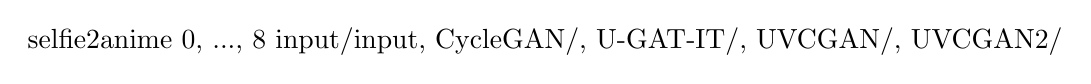
\begin{tikzpicture}
        \node[inner sep=0, fill=white] (G1) at (0, 0) {
            \gridcp{selfie2anime}
                   {0, ..., 8}
                   {input/input, 
                    % ACL-GAN/\aclgan, 
                    % Council-GAN/\council, 
                    CycleGAN/\cyclegan, 
                    U-GAT-IT/\ugatit, 
                    UVCGAN/\uvcgan, 
                    UVCGAN2/\thename}
        };
    \end{tikzpicture}
\end{table*}

\begin{table*}[p]
    \centering
    \caption{\textbf{Sample translations for \animeselfie on \anime.}}
    \label{fig:grid_LQ_animeselfie}
    \tikzexternaldisable
    \tikzsetnextfilename{grid_LQ_anime2selfie}
    \draw[step=1cm, grid-grey,very thick](1,1)grid(8,6); 

\foreach \x in {1,...,8}
	\foreach \y in {1,...,6}
		\draw[grid-grey, fill=white, very thick](\x,\y) circle(0.07cm);
\draw[-stealth, line width=0.85mm] (1.5, 5.9) -- (1.5, 5.1);
    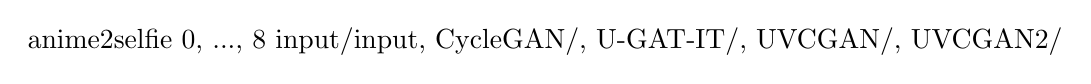
\begin{tikzpicture}
        \node[inner sep=0, fill=white] (G1) at (0, 0) {
            \gridcp{anime2selfie}
                   {0, ..., 8}
                   {input/input, 
                    % ACL-GAN/\aclgan, 
                    % Council-GAN/\council, 
                    CycleGAN/\cyclegan, 
                    U-GAT-IT/\ugatit, 
                    UVCGAN/\uvcgan, 
                    UVCGAN2/\thename}
        };
    \end{tikzpicture}
\end{table*}

\begin{table*}[p]
    \centering
    \caption{\textbf{Sample translations for \malefemale on \celeba.}}
    \label{fig:grid_LQ_malefemale}
    \tikzexternaldisable
    \tikzsetnextfilename{grid_LQ_male2female}
    \draw[step=1cm, grid-grey,very thick](1,1)grid(8,6); 

\foreach \x in {1,...,8}
	\foreach \y in {1,...,6}
		\draw[grid-grey, fill=white, very thick](\x,\y) circle(0.07cm);
\draw[-stealth, line width=0.85mm] (1.5, 5.9) -- (1.5, 5.1);
    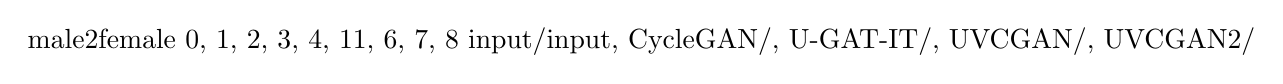
\begin{tikzpicture}
        \node[inner sep=0, fill=white] (G1) at (0, 0) {
            \gridcp{male2female}
                   {0, 1, 2, 3, 4, 11, 6, 7, 8}
                   {input/input, 
                    % ACL-GAN/\aclgan, 
                    % Council-GAN/\council, 
                    CycleGAN/\cyclegan, 
                    U-GAT-IT/\ugatit, 
                    UVCGAN/\uvcgan, 
                    UVCGAN2/\thename}
        };
    \end{tikzpicture}
\end{table*}

\begin{table*}[p]
    \centering
    \caption{\textbf{Sample translations for \femalemale on \celeba.}}
    \label{fig:grid_LQ_femalemale}
    \tikzexternaldisable
    \tikzsetnextfilename{grid_LQ_female2male}
    \draw[step=1cm, grid-grey,very thick](1,1)grid(8,6); 

\foreach \x in {1,...,8}
	\foreach \y in {1,...,6}
		\draw[grid-grey, fill=white, very thick](\x,\y) circle(0.07cm);
\draw[-stealth, line width=0.85mm] (1.5, 5.9) -- (1.5, 5.1);
    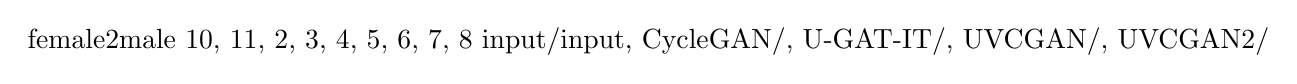
\begin{tikzpicture}
        \node[inner sep=0, fill=white] (G1) at (0, 0) {
            \gridcp{female2male}
                   {10, 11, 2, 3, 4, 5, 6, 7, 8}
                   {input/input, 
                    % ACL-GAN/\aclgan, 
                    % Council-GAN/\council, 
                    CycleGAN/\cyclegan, 
                    U-GAT-IT/\ugatit, 
                    UVCGAN/\uvcgan, 
                    UVCGAN2/\thename}
        };
    \end{tikzpicture}
\end{table*}

\begin{table*}[p]
    \centering
    \caption{\textbf{Sample translations for \rmvGlasses on \celeba.}}
    \label{fig:grid_LQ_rmvGlasses}
    \tikzexternaldisable
    \tikzsetnextfilename{grid_LQ_rmvGlasses}
    \draw[step=1cm, grid-grey,very thick](1,1)grid(8,6); 

\foreach \x in {1,...,8}
	\foreach \y in {1,...,6}
		\draw[grid-grey, fill=white, very thick](\x,\y) circle(0.07cm);
\draw[-stealth, line width=0.85mm] (1.5, 5.9) -- (1.5, 5.1);
    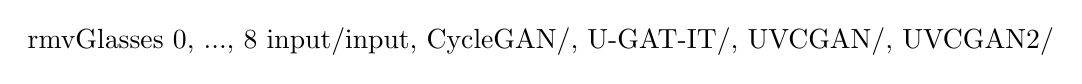
\begin{tikzpicture}
        \node[inner sep=0, fill=white] (G1) at (0, 0) {
            \gridcp{rmvGlasses}
                   {0, ..., 8}
                   {input/input, 
                    % ACL-GAN/\aclgan, 
                    % Council-GAN/\council, 
                    CycleGAN/\cyclegan, 
                    U-GAT-IT/\ugatit, 
                    UVCGAN/\uvcgan, 
                    UVCGAN2/\thename}
        };
    \end{tikzpicture}
\end{table*}

\begin{table*}[p]
    \centering
    \caption{\textbf{Sample translations for \addGlasses on \celeba.}}
    \label{fig:grid_LQ_addGlasses}
    \tikzexternaldisable
    \tikzsetnextfilename{grid_LQ_addGlasses}
    \draw[step=1cm, grid-grey,very thick](1,1)grid(8,6); 

\foreach \x in {1,...,8}
	\foreach \y in {1,...,6}
		\draw[grid-grey, fill=white, very thick](\x,\y) circle(0.07cm);
\draw[-stealth, line width=0.85mm] (1.5, 5.9) -- (1.5, 5.1);
    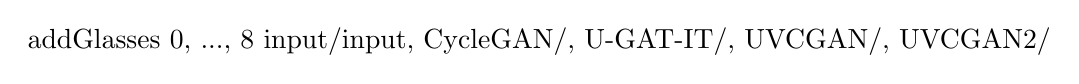
\begin{tikzpicture}
        \node[inner sep=0, fill=white] (G1) at (0, 0) {
            \gridcp{addGlasses}
                   {0, ..., 8}
                   {input/input, 
                    % ACL-GAN/\aclgan, 
                    % Council-GAN/\council, 
                    CycleGAN/\cyclegan, 
                    U-GAT-IT/\ugatit, 
                    UVCGAN/\uvcgan, 
                    UVCGAN2/\thename}
        };
    \end{tikzpicture}
\end{table*}


\def\folder{fig/grid_HQ}

\begin{table*}[p]
    \centering
    \caption{\textbf{Sample translations for \catdog on \afhq.}}
    \label{fig:grid_HQ_catdog}
    \tikzexternaldisable
    \tikzsetnextfilename{grid_HQ_cat2dog}
    \draw[step=1cm, grid-grey,very thick](1,1)grid(8,6); 

\foreach \x in {1,...,8}
	\foreach \y in {1,...,6}
		\draw[grid-grey, fill=white, very thick](\x,\y) circle(0.07cm);
\draw[-stealth, line width=0.85mm] (1.5, 5.9) -- (1.5, 5.1);
    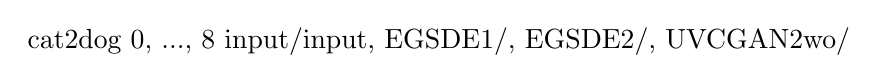
\begin{tikzpicture}
        \node[inner sep=0, fill=white] (G1) at (0, 0) {
            \gridcp{cat2dog}
                   {0, ..., 8}
                   {input/input, 
                    EGSDE1/\egsde, 
                    EGSDE2/\egsdeDG, 
                    UVCGAN2wo/\thename}
        };
    \end{tikzpicture}
\end{table*}

\begin{table*}[p]
    \centering
    \caption{\textbf{Sample translations for \wilddog on \afhq.}}
    \label{fig:grid_HQ_wilddog}
    \tikzexternaldisable
    \tikzsetnextfilename{grid_HQ_wild2dog}
    \draw[step=1cm, grid-grey,very thick](1,1)grid(8,6); 

\foreach \x in {1,...,8}
	\foreach \y in {1,...,6}
		\draw[grid-grey, fill=white, very thick](\x,\y) circle(0.07cm);
\draw[-stealth, line width=0.85mm] (1.5, 5.9) -- (1.5, 5.1);
    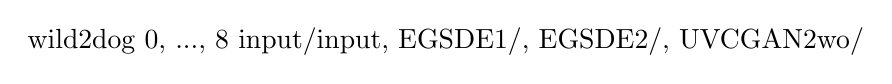
\begin{tikzpicture}
        \node[inner sep=0, fill=white] (G1) at (0, 0) {
            \gridcp{wild2dog}
                   {0, ..., 8}
                   {input/input, 
                    EGSDE1/\egsde, 
                    EGSDE2/\egsdeDG, 
                    UVCGAN2wo/\thename}
        };
    \end{tikzpicture}
\end{table*}

\begin{table*}[p]
    \centering
    \caption{\textbf{Sample translations for \wildcat on \afhq.} 
             Since no benchmarking algorithms studied this task, 
             we only show the input and \thename's translation. }
    \label{fig:grid_HQ_wildcat}
    \tikzexternaldisable
    \tikzsetnextfilename{grid_HQ_wild2cat}
    \draw[step=1cm, grid-grey,very thick](1,1)grid(8,6); 

\foreach \x in {1,...,8}
	\foreach \y in {1,...,6}
		\draw[grid-grey, fill=white, very thick](\x,\y) circle(0.07cm);
\draw[-stealth, line width=0.85mm] (1.5, 5.9) -- (1.5, 5.1);
    \begin{tikzpicture}
        \node[inner sep=0, fill=white] at (0, 0) {
            \begin{tikzpicture}
                \node[inner sep=0] (G1) at (0, 0) {
                    \gridcp{wild2cat}
                           {0, ..., 8}
                           {input/input, UVCGAN2wo/\thename}
                };
                \node[inner sep=0, anchor=north] (G2) at ([yshift=-.1 * \width]G1.south) {
                    \gridcp[9]{wild2cat}
                              {9, ..., 17}
                              {input/input, UVCGAN2wo/\thename}
                };   
            \end{tikzpicture}
        };
    \end{tikzpicture}
\end{table*}

\begin{table*}[p]
    \centering
    \caption{\textbf{Sample translations for \malefemale on \celebahq.}}
    \label{fig:grid_HQ_male2emale}
    \tikzexternaldisable
    \tikzsetnextfilename{grid_HQ_male2female}
    \draw[step=1cm, grid-grey,very thick](1,1)grid(8,6); 

\foreach \x in {1,...,8}
	\foreach \y in {1,...,6}
		\draw[grid-grey, fill=white, very thick](\x,\y) circle(0.07cm);
\draw[-stealth, line width=0.85mm] (1.5, 5.9) -- (1.5, 5.1);
    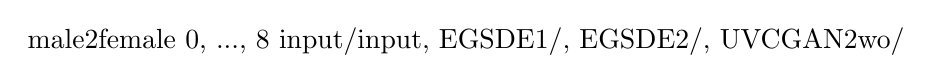
\begin{tikzpicture}
        \node[inner sep=0, fill=white] (G1) at (0, 0) {
            \gridcp{male2female}
                 {0, ..., 8}
                 {input/input, 
                  EGSDE1/\egsde, 
                  EGSDE2/\egsdeDG, 
                  UVCGAN2wo/\thename}
        };
    \end{tikzpicture}
\end{table*}

In this section, we provide additional translation samples to facilitate visual comparison of image quality. 
\autoref{fig:grid_LQ_selfieanime} and \ref{fig:grid_LQ_animeselfie} demonstrate samples on the \anime dataset.
\autoref{fig:grid_LQ_malefemale} and \ref{fig:grid_LQ_femalemale} provide gender swap samples on the \celeba dataset. 
\autoref{fig:grid_LQ_rmvGlasses} and \ref{fig:grid_LQ_addGlasses} show eyeglasses removal and addition samples on the \celeba dataset. 
Finally, \autoref{fig:grid_HQ_catdog}, \ref{fig:grid_HQ_wilddog}, and \ref{fig:grid_HQ_wildcat} provide samples on the \afhq dataset, and \autoref{fig:grid_HQ_male2emale}, \malefemale samples on the \celebahq dataset.
\section{Effects of the Pixel-Wise Consistency Loss}



The main part of the paper compares models trained with two settings of the pixel-wise consistency loss. The \thename model having $\lambda_\text{consist} = 0$ and \thename-C model with $\lambda_\text{consist} = 0.2$. In this section, we show an ablation of the $\lambda_\text{consist}$ values and their effect on the model performance.

\autoref{tab:app_results_lambda_consist} demonstrates the effect of different values of $\lambda_\text{consist}$ on the \thename model realism (as measured by the FID scores) and
pixel-wise faithfulness (as measured by the pixel-wise $L_2$ distance).

As one might expect, the increase in $\lambda_\text{consist}$ is accompanied by an improvement in pixel-wise image faithfulness and a decrease in image
realism. Values of $\lambda_\text{consist}$ below $0.2$ allow one to significantly improve pixel-wise image faithfulness at the expense of a modest loss of image realism. Further increases in $\lambda_\text{consist}$ produce
larger improvements in pixel-wise faithfulness, but also lead to significant decreases in image realism.

Additionally, \autoref{tab:app_results_lambda_consist} demonstrates that the trade-offs of image realism to pixel-wise faithfulness are not uniform across the datasets.
High values of $\lambda_\text{consist}$ allow one to achieve rather large improvements in pixel-wise faithfulness on the \malefemale task at a relatively
small loss of image realism. On the other hand, \catdog translation is subject
to a catastrophic loss of image realism with the increase of $\lambda_\text{consist}$.




\end{document}
